%
\documentclass[11pt,twoside]{article}
\usepackage[letterpaper,margin=1in]{geometry}
\usepackage[utf8x]{inputenc}
\usepackage{amssymb}
\usepackage{graphicx}
\usepackage{verbatim}
\title{Generic Single Edge Fault Tolerant Exact Distance Oracle}
\author{Manoj Gupta\\
   IIT Gandhinagar, India\\
   {\small\texttt{gmanoj@iitgn.ac.in}}
 \and
Aditi Singh\\
   IIT Gandhinagar, India\\
{\small\texttt{aditi.singh@iitgn.ac.in}}
}

\usepackage{amsmath,amssymb,amsthm,xpatch}

%\setlength{\topsep}{0pt}
%\setlength{\partopsep}{0pt plus 0pt minus 0pt}
%\setlength{\parskip}{0pt}
%\setlength{\parindent}{0pt}





\usepackage{dsfont}
\usepackage{xargs}
\usepackage{todonotes}
\usepackage{tikz}
\usepackage[boxruled,lined,linesnumbered]{algorithm2e}
\usepackage{amssymb}
%\usepackage{romannum}
\usepackage{wrapfig}
%\usepackage{mathptmx}
\usepackage{mathrsfs}
\usepackage{enumerate}
\usepackage{caption}
\usepackage{microtype}
\usepackage{soul}
%\usepackage[charter]{mathdesign}
%\usepackage{hyperref}
\usepackage{enumitem}







\newtheorem{theorem}{Theorem}
\newtheorem{lemma}[theorem]{Lemma}
\newtheorem{assumption}[theorem]{Assumption}
\newtheorem{definition}[theorem]{Definition}
\newtheorem{corollary}[theorem]{Corollary}
\newtheorem{observation}[theorem]{Observation}

\newif\iflong
\longtrue

\newcommand{\TT}{\mathcal{T}}
\newcommand{\Ps}{\mathcal{P}}
\newcommand{\conc}{\diamond}
\newcommand{\DET}{\textsc{Detour}}
\newcommand{\UNQ}{\textsc{Unique}}
\newcommand{\FF}{\textsc{First}}
\newcommand{\LL}{\textsc{Last}}
\newcommand{\SBFS}{$\sigma$-\textsc{BFS}}
\newcommand{\BFS}{\textsc{BFS}}
\newcommand{\TZE}{\mathcal{R}_1}
\newcommand{\TON}{\mathcal{R}_1}
\newcommand{\TTW}{\mathcal{R}_2}
\newcommand{\RR}{\mathcal{R}}
\newcommand{\BP}{\mathcal{B}}
\newcommand{\GP}{\mathcal{G}}
\newcommand{\INT}{\textsc{Int}}
\newcommand{\BST}{\textsc{Bst}}
\newcommand{\RMQ}{\textsc{Rmq}}
\newcommand{\HE}{\textsc{Heavy}}
\newcommand{\LI}{\textsc{Light}}
\newcommand{\QQ}{\textsc{Q}}

%\setlength{\textwidth}{6.5in}
%\setlength{\oddsidemargin}{0.0in}
%\setlength{\textheight}{9.2in}
%\addtolength{\topmargin}{-.875in}



\begin{document}



\maketitle

\begin{abstract}
\label{sec:abstract}

%% 1. what is the problem 
Scientific applications that run on leadership computing facilities often face the challenge 
of being unable to fit leading science cases onto accelerator devices due to memory constraints 
(memory-bound applications).
%
% 2. what is your solution 
In this work, the authors studied one such US Department of Energy mission-critical condensed matter 
physics application, Dynamical Cluster Approximation (DCA++), and this paper discusses how device memory-bound challenges were successfully reduced  by proposing an effective 
``all-to-all'' communication method---a ring communication algorithm. 
%
This implementation takes advantage of acceleration on GPUs and remote direct memory access (RDMA) for fast data exchange between GPUs. 
%
\\Additionally, the ring algorithm was optimized with sub-ring communicators
and multi-threaded support to further reduce communication overhead and 
expose more concurrency, respectively.
%
% 3. What's the cherry-picked evaluation result you want to mention
The computation and communication were also analyzed 
by using the Autonomic Performance Environment for Exascale 
(APEX) profiling tool,  and this paper further discusses the 
performance trade-off for the ring algorithm implementation. 
%
The memory analysis on the ring algorithm shows that the allocation size for the authors' most 
memory-intensive data structure per GPU is now reduced to $1/p$ of the original size, where $p$ is the number of GPUs in the ring communicator.
%
The communication analysis suggests that 
the distributed Quantum Monte Carlo execution time grows linearly as sub-ring size increases, and the cost of messages passing through the network interface connector could be a limiting factor.


%
% \todoRed{Ronnie: Next sentence needs rewrite, too much information about Green's function that no one knows in the abstract; recommend generalizing.} \emph {However, DCA++ is currently facing memory-bound challenge as 
% a larger device array $G_t$ is limited by device memory size, where
% $G_t$ is a two-particle Green's function that allows condensed matter
% scientists to explore larger and more complex (higher fidelity)
% physics cases.}

\end{abstract}

\keywords{DCA++, Quantum Monte Carlo, GPU Remote Direct Memory Access, memory-bound issue, exascale machines}

\newpage
Reinforcement learning has achieved great success in areas such as Game-playing \citep{silver2018general,vinyals2019grandmaster}, robotics \cite{kober2013reinforcement}, large language models \citep{ouyang2022training}, etc.
However, due to safety concerns or physical limitations, in some real-world reinforcement learning problems, we must consider additional constraints that may influence the optimal policy and the learning process \citep{garcia2015comprehensive}.
% For example, a robotic arm must not take actions that may cause harm to itself or the environments.
A standard framework to handle such cases is the constrained Markov Decision Process (CMDP) \citep{altman1999constrained}.
Within the CMDP framework, the agent has to maximize
the expected cumulative reward while
obeying a finite number of constraints, which are usually in the form of expected cumulative cost criteria.

However, we are sometimes concerned with the problem with a continuum of constraints.
For example,
the constraints we meet might be time-evolving or subject to uncertain parameters, which
cannot be formulated as an ordinary CMDP
(see Examples \ref{Example_Time_Evolving} and  \ref{Example_Uncertain}).
In this paper we would study a generalized CMDP  
to address the above problem.  Because the constraints are not only infinite-number but also lie
in a continuous set,
the generalization is not trivial. Fortunately, we find that we can borrow the idea behind semi-infinite programming (SIP) \citep{remez1934determination, hettich1993semi} to deal with the semi-infinite constraints.
Accordingly, we propose \emph{semi-infinitely constrained Markov decision processes} (SICMDPs)
as a novel complement to the ordinary CMDP framework.
%More specifically,  an SICMDP model %, we consider 
%contains a continuum of constraints whereas an ordinary CMDP contains a finite number of constraints. 

%This generalization is natural but not trivial. However, we can brows the idea  
%The idea is quite natural and can be backtracked
%to the practice of extending linear programming to linear semi-infinite programming (LSIP) %\cite{remez1934determination, GobernaLSIO1998}.
%In addition, 
%As a complementary approach to the ordinary CMDP framework, 
%SICMDP can be used to model these problems  which cannot be described by a finite number of constraints
%that are not covered by .
%For example,
%the restrictions we consider can be time-evolving or subject to uncertain parameters
%, thus
%cannot be described by a finite number of constraints but a continuum of constraints 
%(see Examples \ref{Example_Time_Evolving} and  \ref{Example_Uncertain}).

We also present two reinforcement learning algorithms to solve SICMDPs called SI-CRL and SI-CPO, respectively.
SI-CRL is a model-based reinforcement learning algorithm designed for tabular cases, and SI-CPO is a policy optimization algorithm for non-tabular cases.
% and analyze its performance both theoretically and empirically.
The main challenge is that we need to deal with a continuum of constraints, thus reinforcement learning algorithms for ordinary CMDPs do not work anymore.
In SI-CRL, we tackle this difficulty by first transforming the reinforcement learning problem to an equivalent LSIP problem, which can then be solved using methods in the LSIP literature like the dual exchange methods \citep{Hu1990,reemtsen1998numerical}.
In SI-CPO, we resort to the idea of cooperative stochastic approximation developed in \cite{lan2020algorithms, wei2020comirror}.
As far as we know, we are the first to introduce tools from semi-infinitely programming (SIP) into the reinforcement learning community for solving constrained reinforcement learning problems.

% To the best of our knowledge, we are the first to apply tools from semi-infinitely programming (SIP) to solve reinforcement learning problems.
Furthermore, we give theoretical analysis for both SI-CRL and SI-CPO.
We decompose the error of SI-CRL into two parts: the statistical error from approximating the true SICMDP with an offline dataset and the optimization error due to the fact that the solution of the LSIP problem obtained by the dual exchange method is inexact.
On the optimization side, we show that the iteration complexity of SI-CRL is $O\left(\left\{\mathrm{diam}(Y)L\sqrt{|\gS|^2|\gA|m}/\left[(1-\gamma)\epsilon\right]\right\}^m\right)$.
On the statistical side, we show that the sample complexity of SI-CRL is $\widetilde O\left(\frac{|S|^2|A|^2}{\epsilon^2(1-\gamma)^3}\right)$ if the offline dataset is generated by a generative model, and $\widetilde O\left(\frac{|S||A|}{\nu_{\min} \epsilon^2(1-\gamma)^3}\right)$ if the dataset is generated by a probability measure $\nu$ as considered in \cite{chen2019information}.
Here $\widetilde O$ means that all logarithm terms are discarded.
For SI-CPO, things become a little more complicated because other than the statistical error and the optimization error, we also need to consider the function approximation error, which comes from imperfect policy parametrizations.
It is shown if the function approximation error can be controlled to $O(\epsilon)$ order, the iteration complexity of SI-CPO is $\widetilde{O}\left(\frac{1}{\epsilon^2(1-\gamma)^6}\right)$ and the sample complexity of SI-CPO is $\widetilde{O}(\frac{1}{\epsilon^4(1-\gamma)^{10}})$.
Here our iteration complexity bound is equivalent to a typical $\widetilde O(1/\sqrt{T})$ global convergence rate.

We perform a set of numerical experiments to illustrate the SICMDP model and validate our proposed algorithms.
Specifically, we examine two numerical examples, namely the discharge of sewage and ship route planning.
Through the discharge of sewage example, we show the advantage of the SICMDP framework over the CMDP baseline obtained by naive discretization in modeling realistic sequential decision-making problems.
Moreover, we demonstrate the effectiveness of the SI-CRL and SI-CPO algorithms in such tabular environments. 
In the ship route planning example, we illustrate the benefits of the SICMDP framework and the ability of the SI-CPO algorithm to address complex continuous control tasks involving continuous state spaces with modern deep reinforcement learning techniques.

% In summary, our contributions are listed as follows.
% First, we present the SICMDP model, which can be viewed as a generalization of the ordinary CMDP model.
% Second, we propose an algorithm to perform reinforcement learning for SICMDPs, which is called SI-CRL, and we believe that we are the first to apply tools from SIP
% to solve reinforcement learning problems.
% Third, we give a theoretical analysis of SI-CRL and identify both its sample complexity and iteration complexity.
% In addition, we perform numerical experiments to illustrate the SICMDP model and validate the SI-CRL algorithm.
% \{This paragraph can be removed!!! \}






We study the problem of selling $m$ items to $n$ buyers. We denote a bundle of items as a quantity vector $\vec{q} \in \Z_{\geq 0}^m$. The number of units of item $i$ in the bundle is $q[i]$. The bundle consisting of only one copy of the $i^{th}$ item is denoted by the standard basis vector $\vec{e}_i$, where $e_i[i] = 1$ and $e_i[j] = 0$ for all $j \not= i$. Each buyer $j \in [n]$ has a valuation function $v_j$ over bundles of items. We denote an allocation as $Q = \left(\vec{q}_1, \dots, \vec{q}_n\right)$ where $\vec{q}_j$ is the bundle that buyer $j$ receives. The cost to produce $\vec{q}$ is $c\left(\vec{q}\right)$ and the cost to produce the allocation $Q$ is $c\left(Q\right)$.
Suppose there are $\kappa_i$ units available of item $i$. Let $K = \prod_{i = 1}^m \left(\kappa_i+1\right)$. We use $\vec{v}_j = \left(v_j\left(\vec{q}_1\right), \dots, v_j\left(\vec{q}_K\right)\right)$ to denote buyer $j$'s values for all of the $K$ bundles and we use $\vec{v} = \left(\vec{v}_1, \dots, \vec{v}_n\right)$ to denote a vector of buyer values. We use the notation $\cX$ to denote the set of all valuation vectors $\vec{v}$. Additive buyers have values $v_j\left(\vec{q}\right) = \sum_{i = 1}^m q[i] v_j\left(\vec{e}_i\right)$ and unit-demand buyers have values $v_j\left(\vec{q}\right) = \max_{i : q[i] \geq 1} v_j\left(\vec{e}_i\right)$. The mechanisms  we study are dominant strategy incentive compatible, so we assume that the bids equal the buyers' valuations.

There is an unknown distribution $\pazocal{D}$ over buyers' values. 
The notation $\profit_M\left(\vec{v}\right)$ denotes the profit of a mechanism $M$ on the valuation vector $\vec{v}$. We use the notation $\profit_{\dist}\left(M\right) = \E_{\vec{v} \sim \dist}\left[\profit_M\left(\vec{v}\right)\right]$ and for a set of samples $\sample$, we use the notation \[\profit_{\sample}\left(M\right) = \frac{1}{|\sample|}\sum_{\vec{v} \in \sample}\profit_M\left(\vec{v}\right).\]

We study real-valued functions parameterized by vectors $\vec{p}$ in $\R^d$, denoted as $f_{\vec{p}}:\domain \to \R.$ For a fixed $\vec{v} \in \domain$, we often consider $f_{\vec{p}}\left(\vec{v}\right)$ as a function of its parameters, which we denote as $f_{\vec{v}}\left(\vec{p}\right)$.
\section{Approach}
\begin{figure}[t]
\centering
\resizebox{0.48\textwidth}{!}{ 
  \includegraphics[width=\textwidth]{figures/workflow.PNG}
}
  \caption{Workflow of \system}
  \label{fig:workflow}
\end{figure}

Figure ~\ref{fig:workflow} shows the overall workflow of \system. The triggers for using \system are usually alert(s) from automated anomaly detection, or sometimes an SRE engineer's suspicion. There are three major steps: constructing the service  dependency graph, constructing the event causality graph,  and root cause ranking. The outputs are the root causes ranked by the likelihood. To support fast human investigation experience, we build an interactive UI as shown in  Figure~\ref{fig:UI}: the service dependency, events with causal links and additional details such as raw metrics or the developer contact (of a code deployment event) are presented to the user for next steps. As an  offline part of human investigation, we label/collect a data set, perform validation, and summarize the knowledge for further improvement on all incidents on a daily basis. %as validations and heterogeneous graph learning (HGL)~\cite{qiao2020heterogeneous} to synthesize the knowledge from existing cases in order to further improve the system.

\subsection{Constructing Service Dependency Graph}
\label{sec:appgraph}

The construction of the service dependency graph starts with the initial alerted or suspicious service(s), denoted as $I$. For example, in Figure ~\ref{fig:ex1_dep}, $I=\{\textit{Checkout}\}$. $I$ can contain multiple services based on the range of the trigger alerts or suspicions. We maintain domain service lists where domain-level alerts can be triggered because there is no clear service-level indication.

At the back end, \system maintains a global service dependency graph $G_{global}$ via distributed tracing and log analysis. The directed edge from nodes $A$ to $B$ (two services or system components) in the dependency graph indicates a service invocation or other forms of dependency. In Figure~\ref{fig:ex1_dep}, the black arrows indicate such edges. Bi-directional edges and cycles between the services can be possible and exist. In this work, the global dependency graph is updated daily.%by extracting from one day's total site traffic.

The service dependency (sub)graph $G$ is constructed using $G_{global}$ and $I$. An extended service list $L$ is first constructed by traversing each service in $I$ over $G_{global}$ for a radius range $r$. Each service $u \in L$ can be traversed by at least one service $v \in I$ within $r$ steps: $L=\{u|\exists v\in I, \ dist(u,v)\le r\ or\ dist(v,u)\le r\}$. Then, the service dependency subgraph $G$ is constructed by the nodes in $L$ and the edges between them in $G_{global}$. In our current implementation, $r$ is set to $2$, since this dependency graph may be dynamically extended in the next steps based on events' detail for longer issue chains or additional dependencies.

\subsection{Constructing Event Causality Graph}
\label{sec:causality}

In the second step, \system collects all supported events for each service in $G$ and constructs the causal links between events. 

\subsubsection{Collecting Events}

Table~\ref{tab:events} presents some example event types and detection techniques for \system's production implementation. For detection techniques, ``De Facto'' indicates that the event can be directly collected via a specific API or storage. %The detection can be done passively at the back end continuously then store anomaly events in different databases; or done actively by pulling data and run detection on the fly to save compute resources. 
The detection either runs passively in the back end to reduce delay and improve accuracy, or runs actively for only the services within the dependency graph range to save resources. %For example, low-level error signals or logs are detected actively since they are too many to scale. 

There are three major categories of events: performance metrics, status logs, and developer activities:
\begin{itemize}
    \item \emph{Performance metrics} represent an anomaly of monitored time series metrics. For example, high CPU usage indicates that the service is causing high CPU usage on a certain machine. In this category, most events are continuously and passively detected and stored. %For high CPU usage, threshold indicates the event is created when CPU usage is higher than certain predefined value. TPS spike indicates a spike in transaction per second, since TPS is a moving average value, we use some statistical model learned from historical data to detect such events.
    \item \emph{Status logs} are caused by abnormal system status, such as spike of HTTP error code metrics while accessing other services' endpoints. Different types of error metrics are important and supported in \system, including third-party APIs. For example, Bad Host indicates abnormal patterns on some machines running the service, and can be detected by a  clustering-based ML approach.%Markdown indicates that the whole service is down. 
    \item \emph{Developer activities} are the events generated when a certain activity of developers is triggered, such as code deployment and config change.
\end{itemize}

\begin{table}[t]
\centering
\caption{List of example event types used in \system}
\resizebox{0.4\textwidth}{!}{ 
\begin{tabular}{|c|c|c|}
\hline
Type                                & Event Type                  & Detection Technique  \\ \hline
\multirow{6}{*}{Performance Metrics} & High GC (Overhead)      & Rule-based        \\ \cline{2-3} 
                                    & High CPU Usage          & Rule-based        \\ \cline{2-3} 
%                                    & Out of Memory           & Rule-based        \\ \cline{2-3} 
%                                    & LB Connection Stacking  & Statistical Model \\ \cline{2-3} 
                                    & Latency Spike           & Statistical Model \\ \cline{2-3} 
                                    & TPS Spike               & Statistical Model \\ \cline{2-3} 
                                    & Database Anomaly        & ML Model          \\ \cline{2-3} 
                                    & Business Metric Anomaly & ML Model          \\ \hline
\multirow{4}{*}{Status Logs}        & WebAPI Error            & Statistical Model \\ \cline{2-3} 
                                    & Internal Error          & Statistical Model \\ \cline{2-3} 
                                    & ServiceClient Error     & Statistical Model \\ \cline{2-3} 
                                    & Bad Host                & ML Model          \\ \hline %\cline{2-3} 
%                                    & Hystrix Circuit Break   & De Facto          \\ \hline
\multirow{3}{*}{Developer Activities} & Code Deployment         & De Facto          \\ \cline{2-3} 
                                    & Configuration Change    & De Facto          \\ \cline{2-3} 
                                    & Execute URL             & De Facto          \\ \hline
\end{tabular}
}
\label{tab:events}
\end{table}

In Groot, there are more than a dozen event types such as \emph{Latency Spike} as listed in the column 2 of Table~\ref{tab:events}. 
Each event type is characterized by three aspects: $Name$ indicates the name of this event type; $Lookback Period$ %\footnote{In Figure~\ref{fig:ex2_n1}, there are two periods, 1 day indicates the look-back range if the model has already finished deployment, 4 days indicates the range if the model deployment is still ongoing(incremental deployment).} 
indicates the time range to look back (from the time when the use of \system is triggered) for collecting events of this event type;  $PropertyType$ indicates the types of the properties that an event of this event type should hold. 
$PropertType$  is characterized by a vector of pairs, each of which indicates the string type for a property's name and the primitive type for the property's value such as string, integer, and float. 
Formally, an event type is defined as a tuple: 
$ET = <Name, Lookback Period, PropertyType>$ 
where 
$PropertyType = <(string, \textit{type}_1), ..., (string, \textit{type}_{n})>$ ($n$ is the number of properties that an event of this event type holds). 
%

Each event of a certain event type $ET$ is characterized by four aspects:
$\textit{Service}$ indicates the service name that the event belongs to; $\textit{Type}$ indicates $ET$'s $\textit{Name}$;  $\textit{StartTime}$ indicates the time when the event happens; $\textit{Properties}$ indicates the properties that the event  holds.
Formally, an event is defined as a tuple: 
$e = <Service, Type, StartTime, Properties>$ 
where $Properties$ is an instantiation of $ET$'s  $PropertyType$. 


%and each event is defined as $e = \{<\textit{Property}_i, \textit{value}_i>\}$. Each event type serves as a template for the event instantiation. such as a string, an integer, a float or a set of primitive types while $\textit{value}$ is limited to primitive data types. 
%
%Each event is defined as a sequence of property-value pairs where the set size is $n$.

For example, in Figure~\ref{fig:example1}, the generated event for \emph{Latency Spike in DataCenter-A} in \emph{Service-C} would be $<``\textit{Service-C}'', ``\textit{Latency\ Spike}'', \textit{2021/08/01-12:36:04}, <(``\textit{DataCenter}'',``\textit{DC-1}''),  ...>>$. %So for each service in $G$, we detect/collect and filter the events within specified time range of the alert.

\subsubsection{Constructing Causal Link}

After collecting all events on all services in $G$, in this step, causal links between these events are constructed for RCA ranking. The causal links (red arrows) in Figure~\ref{fig:ex1_cas} are such examples. A causal link represents that the source event can possibly be caused by the target event. SRE knowledge is engineered into rules and used to create causal links between the pairs of events. %As shown in Figure~\ref{fig:example2}, there are two categories of rules: basic rules and conditional rules. 

A rule for constructing a causal link is defined as a tuple:  $Rule = <Target\mbox{-}Type,  Source\mbox{-}Events, Target\mbox{-}Events, Direction,\\ Target\mbox{-}Service,  Condition>$  ($Condition$ can be optionally specified). $Target\mbox{-}Type$ indicates the type of the rule, being either $Static$ or $Dynamic$ (explained further later). $Source\mbox{-}Events$ indicates the type of the causal link's source event ($Source\mbox{-}Events$ are listed in the names of the rules shown in Figures~\ref{fig:ex2_n1},~\ref{fig:ex2_n2} and~\ref{fig:dynamic_example}).   $Target\mbox{-}Events$ indicates the type of the causal link's target event. $Direction$ indicates the direction of the casual link between the target event and source event. $Target\mbox{-}Service$ indicates the service that the target event should belong to. Note that $Target\mbox{-}Service$ in $Static$ rules can be  $Self$, which indicates that the target event would be within the same service as the source event, or $Outgoing$/$Incoming$, which indicates that the target event would belong to the downstream/upstream services of the service that the source event belongs to in $G$.

\begin{figure}[t]
\centering
\includegraphics[width=0.56\columnwidth]{figures/example3.png}
\caption{Example of dynamic rule}
\label{fig:dynamic_example}
\end{figure}

There are two categories of special rules. The first category is \emph{dynamic} rules (i.e., rules whose $Target\mbox{-}Type$  is set to $Dynamic$) to support dynamic dependencies. Here $Target\mbox{-}Service$ does not indicate any of the three possible options listed earlier but indicates the name of the target service that \system would need to create. For example, live DB dependencies are not available due to different tech stacks and high volume. In Figure~\ref{fig:dynamic_example}, a DB issue (DB Markdown) is shown in \emph{Service-A}. Based on the listed \emph{dynamic} rule, \system creates a new ``service'' \emph{DB-1} in $G$, a new event ``Issues'' that belongs to \emph{DB-1}, and a causal link between the two events.  In practice, the SRE teams use dynamic rules to cover a lot of third-party services and database issues since the live dependencies are not easy to maintain.  %However through the internal error messages and dynamic rules, \system is still able to handle these dependencies. %we can still support external inferences. 

The second category of special rules is \emph{conditional} rules. \emph{Conditional} rules are used when some prerequisite conditions should be satisfied before a certain causal link is created. In these rules, $Condition$ is specified with a boolean predicate. As shown in Figure~\ref{fig:ex2_n2}, the SRE teams believe \emph{Latency Spike} events from different services are related only when both events happen within the same data center. Based on this observation, \system would first evaluate the predicate in $Condition$ and build only the causal link when the predicate is true. A conditional rule overwrites the basic rule on the same source-target event pair.

When constructing causal links, \system first applies the \emph{dynamic} rules so that dynamic dependencies and events are first created at once. Then for every event in the initial services (denoted as $I$), if the rule conditions are satisfied, one or many causal links are created from this event to other events from the same or upstream/downstream services. When a causal link is created, the step is repeated recursively for the target event (as a new origin) to create new causal links. After no new causal links are created, the construction of the event causality graph is finished.

% When \system constructs the causal links, \system first processes all dynamic rules as they may create new event nodes in the graph. %\system enumerates the dynamic rules on each existing event node and also on the newly added nodes (There could also be rules applicable to the newly added nodes) until no new event nodes can be created. 


%Each rule is defined as a predicate containing both events' property-value pair. If the predicate evaluates to be true between two events, then we would add the edge in the causality graph. For example, in Figure~\ref{fig:example1}, the rule used to establish the edge between \emph{GC overhead in RNO} and \emph{Latency increase in LVS, RNO, SLC} would be like this: Suppose we are now determining whether there should be a link from event $u$ to event $v$, then this rule would be $u.\text{pool} = v.\text{pool}\ and\ u.\text{type} = ``\text{High GC Overhead}"\ and\ v.\text{type} = ``\text{Latency increase}"\ and\ u.\text{center} \cap v.\text{center} \ne \emptyset$ which holds true for these two events. Each causality link is also associated with a weight which represents the likelihood of causality - we set all initial values as $1.0$. Overtime these value are updated by the statistical analysis result of the collected data set.


\subsection{Root Cause Ranking}
Finally, \system ranks and recommends the most probable root causes from the event causality graph. Similar to how search engines infer the importance of pages by page links, we customize the PageRank \cite{manning2010introduction} algorithm to calculate the root cause ranking; the customized algorithm is named as GrootRank. The input is the event causality graph from the previous step. Each edge is associated with a weighted score for weighted propagation. The default value is set as $1$, and is set lower for alerts with high false-positive rates. 

Based on the observation that dangling nodes are more likely to be the root cause, we customize the personalization vector as $P_n = f_n $ or $P_d = 1$, where $P_d$ is the personalization score for dangling nodes, and $P_n$ is for the remaining nodes; and $f_n$ is a value smaller than 1 to enhance the propagation between dangling nodes. In our work, the parameter setting is $f_n = 0.5$, $\alpha = 0.85$, $max_{iter} = 100$ (which are parameters for the PageRank algorithm). Figure \ref{fig:person} illustrates an example. The grey circles are the events collected from three services and one database. The grey arrows are the dependency links and the red ones are the causal links with the weight of $1$. Both of the PageRank and GrootRank algorithms detect $event 5$ (DB issue) as the root cause, which is expected and correct. However, the PageRank algorithm ranks $event 4$ higher than $event 3$. But $event 3$ of $\textit{Service-C}$ is more likely to be the second most possible root cause (besides $event 5$), because the scores on dangling nodes are propagated to all others equally in each iteration. We can see that $event 3$ is correctly ranked as second using the GrootRank algorithm.

The second step of GrootRank is to break the tied results from the previous step. The tied results are due to the fact that the event graph can contain multiple disconnected sub-graphs with the same shape. We design two techniques to untie the ranking: 
\begin{figure}[t]
\centering
  \includegraphics[width=0.8\columnwidth]{figures/personalvector.png}
  \caption{Example of personalization vector customization}
  \label{fig:person}
\end{figure}

\begin{figure}[t]
\centering
  \includegraphics[width=0.8\columnwidth]{figures/accessdistance.png}
  \caption{Example of using access distance to untie the ranking results}
  \label{fig:untie}
\end{figure}
\begin{enumerate}
\item For each joint event, the access distance (sum) is calculated from the initial anomaly service(s) to the service where the event belongs to. If any ``access'' is not reachable, the distance is set as $d_m+1$ where $d_m$ is the maximum possible distance. The one with shorter access distance (sum) would be ranked higher and vice versa. Figure \ref{fig:untie} presents an example, where \emph{Service-A} and \emph{Service-B} are both initial anomaly services. Since \system suspects that $event 2$ is caused by either $event 3$ or $event 1$ with the same weight. The scores of $event 3$ and $event 1$ are tied. Then, $event 3$ has a score of $1$ (i.e., $0+1$) and $event 1$ has a score of 2 (i.e., $0+2$), since it is not reachable by \emph{Service-B}). Therefore, $event 3$ is ranked first and logical. 
\item For the remaining joint results with the same access distances, \system continues to untie by using the historical root cause frequency of the event types under the same trigger conditions (e.g., checkout domain alerts). This frequency information is generated from the manually labeled dataset. A more frequently occurred root cause type is ranked higher.% than the less frequent ones.
\end{enumerate}


\subsection{Rule Customization Management}

While \system users create or update the rules,  there could be overlaps, inconsistencies, or even conflicts being introduced such as the example in Figure~\ref{fig:ex2_n2}. \system uses two graphs to manage the rule relationships and avoid conflicts for users. One graph is to represent the link rules between events in the same service (\emph{Same-Graph}) while the other is to represent links between different services (\emph{Diff-Graph}). The nodes in these two graphs are the event types defined in Section~\ref{sec:causality}. There are three statuses between each (directional) pair of event types: (1) no rule, (2) only basic rule, and (3) conditional rule (since it overwrites the basic rule). In \emph{Same-Graph}, \system does not allow self-loop as it does not build links between an event and itself.
% but it is possible that we build links between different services with the same event type.

When rule change happens, existing rules are enumerated to build edges in \emph{Same-Graph} and \emph{Diff-Graph} based on $Target\mbox{-}Events$ and $Target\mbox{-}Service$. Based on the users' operation of 
% \begin{itemize}
%     \item 
    (1) ``remove a rule'',  \system removes the corresponding edge on the graphs;
    % \item 
    (2) ``add/update a rule'',  \system checks whether there are existing edges between the given event types, and then warns the users for possible overwrites. 
    % The users can also combine the conditional rules.   % while users are adding basic rules between event types if there are existing conditional rules between them.
    If there are no conflicts, \system just adds/updates edges between the event types.
    % \item Add conditional rules. We would first alert the possible overwrite. Then if users are about to add new conditional rules on the top of existing conditional rules, we would ask the users to combine these two conditions to add a new one. We then build or change all corresponding edges to status 3.
% \end{itemize} 

After all changes, \system extracts the rules from the graphs by converting each edge to a single rule. These rules are automatically implemented, and then tested against our labeled data set. The \system users need to review the changes with validation reports before the changes go online.

% Note that currently we don't check the consistencies between dynamic rules as we cannot process the dynamic event types, but this could be solved in the future by using nodes with symbolic values to represent such event types. 

% !TEX root = paper.tex
\iflong
\else
\vspace{-2mm}
\fi
\section{Preferred replacement path passes through $t_s$}
\label{sec:passes}
\iflong
Under this assumption, we only need to find the preferred replacement path from $s$ to $t_s$ avoiding $e$. Note that we already know $|t_st|$ length via $B_0(t_{s},t)$. We use the following additional data structures:



\begin{itemize}[leftmargin=*,noitemsep,nolistsep]
\item $B_2$: For $x \in S \cup \TT$ and $y \in V$, $B_2(x,y)$ contains the vertex $w$ on $xy$ path such that $|yw| = 2^{\lfloor \log |xy| \rfloor}$, or in words, the vertex nearest to $x$ whose distance from $y$ is a power of 2. The size of $B_2$ is $\tilde O((\sigma+\sqrt{n\sigma})n) = \tilde O(\sigma^{1/2}n^{3/2})$.

\item $B_3$: For $x \in V$ and $y \in \TT$, $B_4(x,y, \oplus2^i)$
contains the shortest path from $x$ to $y$ avoiding every
$2^i$-th
edge on the path $xy$ from $x$ (where $i \le \log \lfloor
|xy| \rfloor$). Since $|\TT| = \tilde O(\sqrt{n \sigma})$, the size
of $B_3$ is $\tilde O( \sigma^{1/2} n^{3/2} )$.

\item $B_4$: For $s \in S$ and $x \in V$, $B_4(s,x, \ominus2^i)$ contains  the shortest path from $s$ to $x$ avoiding the $2^i$-th
edge on the path $sx$ from $x$ (where $i \le \log \lfloor |sx| \rfloor$). The size of $B_4$ is $ \tilde O( n \sigma) = \tilde O( \sigma^{1/2} n^{3/2} )$.



\item $B_5$: For every $s \in S$ and $x \in \TT$, $B_5(s,x, [\oplus 2^i, \ominus 2^j])$ contains the shortest path from $s$ to $x$ avoiding the sub path
that start from $2^i$-th vertex from $s$ and ends at $2^j$-th
vertex from $x$ on the path $sx$ (where  $i,j \le \log \lfloor sx \rfloor$). The size of $B_5$ is $\tilde O(\sigma^{3/2} n^{1/2}) = \tilde O( \sigma^{1/2} n^{3/2} )$.


\end{itemize}

\begin{figure}
\centering

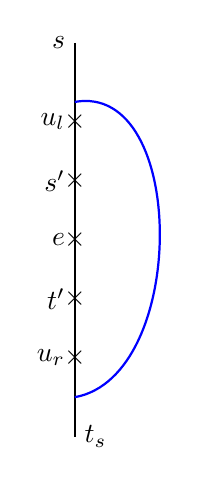
\begin{tikzpicture}[scale=1]

\coordinate (x) at (0,5);
\coordinate (y) at (0,0);
\coordinate (u) at (0,2.5);
\coordinate (ul) at (0,1);
\coordinate (ur) at (0,4);

\coordinate (x1) at (0,1.75);
\coordinate (y1) at (0,3.25);

\draw[thick](x)--(y);
\node[left] at (x){$s$};
\node[right] at (y){$t_{s}$};

\node[left] at (u){$e$};
\node at (u){$\times$};
\node[left] at (ul){$u_r$};
\node at (ul){$\times$};
\node[left] at (ur){$u_l$};
\node at (ur){$\times$};

\node[left] at (x1){$t'$};
\node at (x1){$\times$};
\node[left] at (y1){$s'$};
\node at (y1){$\times$};

\draw[thick,blue] (0,0.5) to[out=10,in=10] node[pos=0.2,
left]
{ } (0,4.25);
\end{tikzpicture}
\caption{The hardest part of the distance oracle, when the
replacement path neither passes through $u_l$ not $u_r$.}
\end{figure}

\noindent   Assume that we get a query
{\sc Q}($s,t,e(u,v)$), that is, find the shortest path from
$s$ to $t$ avoiding $e$. Assume without loss of generality that $u$ is closer to $s$ on $st$ path than $v$. We answer this query as follows:
first we find the distance of $v$ from $s$, via $B_0(s,v)$. If $B_0(s,v)$ is a power of 2 then
we can directly use $B_3(s,t_s, \oplus |sv|) + B_0(t_s,t)$. Else, let $u_l \leftarrow  B_2(s,v)$ and
$u_r \leftarrow B_2(t_s,u)$. Here $u_l$ is the nearest vertex to $s$ on $vs$ path whose
 distance from $v$ is a power of 2. Similarly, $u_r$ is the nearest vertex to $t_s$ on $ut_s$ path whose distance form $u$ is a power of 2.    There are three cases now:

\begin{enumerate}[noitemsep,nolistsep]
\item  The  preferred replacement path passes through $u_l$.

\item  The preferred replacement path passes through $u_r$.

\item The preferred replacement path neither passes through $u_l$
nor $u_r$.

\end{enumerate}
\noindent For the first case, we  can report $B_0(s,u_l) + B_3(u_l, t_{s}, \oplus|u_lv|) + B_0(t_s,t) $. For the second case, we can report $B_4(s,u_r, \ominus  |uu_r|) + B_0(u_r,t_s) + B_0(t_s,t)$ . The hardest
case is when the preferred replacement path neither passes through
$u_l$ nor $u_r$. Let $s'$ be the farthest
vertex  on $sv$ path from $s$ whose distance is a power
of 2, that is $|ss'| = 2^{\lfloor \log |sv| \rfloor}$. Similarly let $t'$ be the farthest vertex on $t_{s}u$
path from $t_s$ whose distance is a power
of 2. Now,
we can  report the shortest path from $s$ to $t_{s}$ avoiding
$[s',t']$ -- this is also stored in $B_5(s,t_s,[\oplus 2^{\lfloor \log |sv| \rfloor}, \ominus 2^{\lfloor
\log |t_su| \rfloor}] )$. By construction, if the shortest path avoids $[u_l,u_r]$, then it also
avoids $[s',t']$. Thus we can return $B_5(s,t_s,[\oplus 2^{\lfloor \log |sv| \rfloor}, \ominus 2^{\lfloor
\log |t_su| \rfloor}] ) +\ B_0(t_s,t)$ as the length  of the preferred replacement path.
The reader can check that the running time of our algorithm
is $O(1)$ as we have to check $B_0,B_1,B_2,B_3,B_4,B_5$ constant number of times.
For the correctness of the above procedure, please refer to \cite{DemetrescuTCR08,DuanP09}.
\else
Since this case is a generalization of the techniques developed by
Demetrescu et. al. \cite{DemetrescuTCR08}, concerned reader may read
the full version of the paper for details -- where we show that there exists a data-structure
of size $\tilde O(\sigma^{1/2}n^{3/2})$ which takes $O(1)$ time to find a replacement
path from $s$ to $t$ that avoids $e$ but passes through $t_s$.
\fi

Now, we move on to the harder case, that is, replacement paths avoid $t_s$ too. For this, we will  fix a vertex $t$. We will show
that the query
${\sc Q}(s,t,e(u,v))$  can be answered
in $\tilde O(1)$ using $\tilde O(\sqrt{\sigma n})$ space.
This immediately implies that we can answer exact queries
in $\tilde O(1)$ time using $\tilde O(\sigma^{1/2} n^{3/2})$
space.

%In the rest of the paper, we try to find a distance
%oracle for a fixed $t$.

% !TEX root = paper.tex
\iflong
\else
\vspace{-2mm}
\fi
\section{Preferred Replacement path avoids $t_s$}

\label{sec:avoids}


Handling preferred replacement paths that avoid $t_s$ turns out to be a challenging and unexplored case. For better exposition, we will first solve the problem for the case when $\sigma=1$, that is there is only one source.
Let $\RR$ be the set of all preferred replacement paths from $s$ to $t$ that do not pass through $t_s$. We make  two important observations:

\begin{enumerate}[noitemsep,nolistsep]

\item The size of $\RR$ is $ O(\sqrt n)$.

\item Preferred replacement paths in $\RR$ avoid one contiguous sub path of $st$.

\end{enumerate}

\noindent Few remarks are in order. If the preferred replacement paths in $\RR$ were disjoint, then bounding the size of $\RR$ is easy. However, we are able to bound the size of $\RR$ even if paths are intersecting.  The second observation implies that we can build a balanced binary search tree containing paths in $\RR$. Each node in this tree will contain a preferred replacement path $P$. The key for each node will be the start and end vertex of the sub path $P$ avoids.  We will use this BST to find an appropriate replacement path that avoids an edge $e$.

\begin{definition}(Detour of a replacement path)
Let $P$ be a preferred replacement path avoiding an edge $e$ on $st$ path. Then detour of $P$ is defined as, $\DET(P) := P \setminus st$. That is, detour is a path the leaves $st$ before $e$ till the point it merges back to $st$ again.
\end{definition}

\begin{comment}
\begin{lemma}
\label{lem:prop}
Let $P$ be a replacement path in $\RR$ that avoids $u$ on $st_s$ path. Then
 $P$ can merge back to $st$ path just once.
\end{lemma}
\begin{proof}
Since $P$ is a replacement path from $s$ to $t$ avoiding $u$, it necessary has to merge somewhere on path $st$. Assume that $P$ merges back at $w$ on $st$ path. Note that $w$ cannot lie before $u$ on $st$ path as the sub-path $sw$ of the $st$ path is the shortest path from $s$ to $w$. This implies that $w$ lies after $u$ on $st$ path. After merging at $w$, $P$ can continue on the sub path $wt$ (of path $st$) to reach $t$, as this is the shortest path from $w$ to $t$.
\end{proof}
\end{comment}
\noindent Since our  replacement path $P$  also avoids $t_s$, the following lemma is immediate by the definition of preferred path.

\begin{lemma}
Let $P$ be a preferred replacement path in $\RR$ that avoids $e$ and $t_s$ on
$st$ path, then (1) $\DET(P)$ cannot merge back to $st_s$ path and (2) $\DET(P)$ is a contiguous path.
\end{lemma}
\begin{lemma}
\label{lem:avoids}
Let $P,P' \in \RR$ avoid $e$ and $e'$ respectively on $st_s$ path. Also assume that $e$ is closer to $s$ than $e'$. Then
(1)  P avoids $e'$  (2) $\DET(P')$ starts  after $e$ on $st_s$ path and (3) $|P| > |P'|$.

\end{lemma}

\iflong
  \begin{proof}

  \noindent (1) $P$ diverges from $st_s$ path above $e$. Since $P
  \in \RR$, it   merges back on $t_st$ path only. Since $e,e'
  \in st_s$ (we are in {\em far} case) and $e$ is closer to $s$ than $e'$, this implies
  that $P$ also avoids $e'$.

  \noindent (2) Assume that  $\DET(P')$ starts above $e$ on
  $st_s$ path. This implies that both $P$ and $P'$ avoid $e$
  and $e'$. But then, our algorithm will choose one of these two paths as a preferred path that avoids both $e$ and $e'$.  Thus,
  we arrive at a contradiction as there are two different preferred replacement paths avoiding $e$ and $e'$.

  \noindent (3) Since $P$  avoids $e'$ (by (1)) and $\DET(P')$ starts after $e$ (by (2)), $P'$ is the preferred path to avoid $e'$ only if $|P'| < |P|$ (else $P$ would be the preferred path as it leaves the $st$ path earlier than $P'$).



  \end{proof}
\fi

\noindent The converse of the third part of the lemma is also true. Since we will be using it in future, we prove it now.

\begin{lemma}
\label{lem:avoidreverse}

Let   $P$ and $P'$ be two preferred replacement paths that avoid $e$ and $e'$ on $st$ path respectively. If $|P| > |P'|$, then $e$ is closer to $s$ than $e'$.
\end{lemma}

\iflong
  \begin{proof}
  Assume for contradiction that $e'$ is closer to $s$ than $e$. Since the replacement path $P'$ has to diverge from $st$ before $e'$ and merge again only in $t_st$,  $P'$ also avoid $e$. But then $P'$ should be the replacement path for avoiding $e$ too, as $|P'| < |P|$, a  contradiction.
  \end{proof}
\fi
\iflong
\else
\begin{figure}[hpt!]
\centering
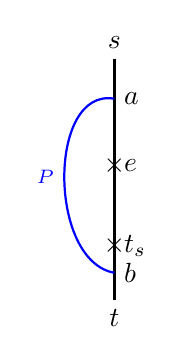
\begin{tikzpicture}[scale=1.7]

\definecolor{dgreen}{rgb}{0.0, 0.5, 0.0}
\begin{scope}[xshift=0cm]
\coordinate (s) at (0,1.8);
\coordinate (t) at (0,0);
\coordinate (ts) at (0,0.4);
\coordinate (b) at (0,.2);

\coordinate (a) at (0,1.5);
\coordinate (v) at (0,1);

\draw[thick](s)--(t);
\node[above] at (s){$s$};
\node[below] at (t){$t$};
\node[right] at (a){$a$};
\node[right] at (b){$b$};



\draw[blue,thick] (a) to[out=170,in=170] node[pos=0.5,left]
{\scriptsize  $P$}  (b);
\node at (v){$\times$};
\node[right] at (v){$e$};

\node at (ts){$\times$};
\node[right] at (ts){$t_s$};
\end{scope}

\end{tikzpicture}

\caption{$\DET(P)$ does not intersect detour of any path in $(>P)$}
\label{fig:singlefirstcase}
\end{figure}

\fi
\noindent By Lemma \ref{lem:avoids}{\small(3)}, we know that all preferred replacement
paths in $\RR$ have different lengths. In fact, it is the main reason we defined a preferred replacement path. We can thus arrange
these paths   in decreasing order of their lengths. Thus, we get the following corollary.
\begin{corollary}
\label{cor:arrange}
 Given a set $\RR$ of preferred replacement paths from $s$ to $t$ (that also avoid $t_s$), we can arrange  paths in decreasing order of their lengths.
\end{corollary}

\noindent Given a path $P \in \RR$, let $(<P)$ be the set of all preferred replacement paths with length less than $P$. Similarly, let $(>P)$ be the set of all preferred replacement paths with length greater than $P$.   If $P$ avoids $e$, then by Lemma \ref{lem:avoidreverse}, it also avoids all  edges avoided by paths in $(<P)$.  By Lemma \ref{lem:avoids}, for any path $P' \in (<P)$, $\DET(P')$ starts after $e$ on $st_s$ path.
We will now show a simple but important property of a path $P$ in $\RR$.

\begin{lemma}
\label{lem:length}
Let $P \in \RR$ be the shortest path from $s$ to $t$ avoiding $e$ such that $|P| = |st| +\ \ell$ where $\ell \ge 0$, then the size of the set $(<P)$ is $\le \ell$.
\end{lemma}
\iflong
  \begin{proof}
  Since a path in $(<P)$ avoids some edge in $st$ path, its length has to be $\ge |st|$. By Corollary \ref{cor:arrange},
  all paths in $\RR$, and thus $(<P)$ have different lengths. But the length of paths in $(<P)$ is less than the length of $P$.
  Thus, there can be atmost $\ell$ paths in $(<P)$.
  \end{proof}
\fi

\begin{definition}
\label{def:unique}
(Unique path of $P$) Let $\UNQ(P)$ be the prefix of\ $\DET(P)$ which does not intersect with any detours in $\cup_{P' \in (>P)} \DET(P')$.
\end{definition}
%Note that $\UNQ(P)$ can be an empty path too.
We now arrange all  preferred replacement paths in $\RR$ in decreasing order of their lengths. Assume that we are processing a path $P$ according to this ordering such that $P$ avoids $e$ on $st$ path. If $|\UNQ(P)| \ge \sqrt n$, then we have associated $O(\sqrt n)$ vertices on $\UNQ(P)$ to $P$. Else $\UNQ(P) < \sqrt{n}$ and we have the following two cases:

\iflong
\else
\vspace{-2mm}
\fi
\subsection{   $\DET(P)$ does not intersect with  detour of any path in $(>P)$}
\label{subsec:singlecaseone}
\iflong
\begin{figure}[hpt!]
\centering
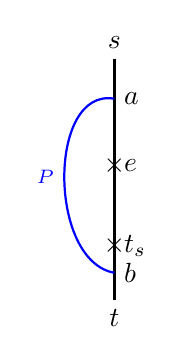
\begin{tikzpicture}[scale=1.7]

\definecolor{dgreen}{rgb}{0.0, 0.5, 0.0}
\begin{scope}[xshift=0cm]
\coordinate (s) at (0,1.8);
\coordinate (t) at (0,0);
\coordinate (ts) at (0,0.4);
\coordinate (b) at (0,.2);

\coordinate (a) at (0,1.5);
\coordinate (v) at (0,1);

\draw[thick](s)--(t);
\node[above] at (s){$s$};
\node[below] at (t){$t$};
\node[right] at (a){$a$};
\node[right] at (b){$b$};



\draw[blue,thick] (a) to[out=170,in=170] node[pos=0.5,left]
{\scriptsize  $P$}  (b);
\node at (v){$\times$};
\node[right] at (v){$e$};

\node at (ts){$\times$};
\node[right] at (ts){$t_s$};
\end{scope}

\end{tikzpicture}

\caption{$\DET(P)$ does not intersect detour of any path in $(>P)$}
\label{fig:singlefirstcase}
\end{figure}

\fi
    Let $\DET(P)$ start at $a$ and end at $b$ -- the vertex where it touches
    $t_st$ path. Let $ab$ denote the
path from $a$ to $b$ on $P$. By our assumption $\UNQ(P) = ab$ and $|ab| < \sqrt n$.
    By Lemma \ref{lem:avoids}, all  replacement paths in $(<P)$ pass through $e$
    (as detour of these replacement paths start below $e$) and by Lemma \ref{lem:avoidreverse},
    these replacement paths avoid edges that are closer to $t$ than $e$. We can view the
    replacement paths as if they are starting from the vertex $a$. That is, consider  paths
    $\{P\setminus sa\} \cup \{ P'\setminus sa | \ P' \in (<P)\}$. These replacement
    paths avoid edges in $at$.   $|P \setminus sa| = |ab| +  |bt| \le |ab|\ + |at| < |at| + \sqrt n$.
    Applying Lemma \ref{lem:length}, we infer that the number of paths in $\{ P'\setminus
sa | P' \in (<P)\}$ is $\le \sqrt n$

\iflong
\else
\vspace{-2mm}
\fi
\subsection{$\DET(P)$ intersects with  detour of a path in $(>P)$}
\label{subsec:singlecasetwo}
Assume that $P$ first intersects with $P' \in (>P)$. Let $P'$ avoid $e'$ and $\DET(P')$ start at $a'$ and end at $b'$ (see Figure \ref{fig:singlesecondcase}). Let us assume that $\DET(P)$ starts at $a$ and it intersects $\DET(P')$ at $c$. This implies that $\UNQ(P) = ac$.

\noindent Consider the path $sa' \conc a'c \conc ca \conc at$. We claim that this path avoids $e'$. This is due to the fact that by Lemma \ref{lem:avoids}, $\DET(P)$
starts after $e'$ on $st$ path. So, $ca$ and $at$ avoids $e'$. Since $P' = sa' \conc a'c \conc cb' \conc b't$, length of $P'$ must be $\le$ length of the alternate path. Thus,\\
\begin{tabular}{llll}
 & $|sa'| +  |a'c|
+ |cb'| + |b't|$  & $\le$ &$|sa'| + |a'c| + |ca|  + |at|$\\
$\implies$& $
|cb'| + |b't|$ & $\le$ & $|ca|  + |at|$   \\
$\implies$& $|ac| +
|cb'| + |b't|$ & $\le$ &   $2|ca|  + |at|$

\end{tabular}

\begin{figure}[hpt!]
\centering
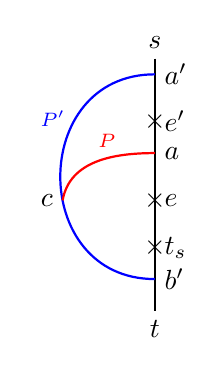
\begin{tikzpicture}[scale=2]

\definecolor{dgreen}{rgb}{0.0, 0.5, 0.0}
\begin{scope}[xshift=0cm]
\coordinate (s) at (0,1.6);
\coordinate (t) at (0,0);
\coordinate (ts) at (0,0.4);
\coordinate (b1) at (0,.2);

\coordinate (a1) at (0,1.5);
\coordinate (a) at (0,1);
\coordinate (v) at (0,0.7);
\coordinate (v1) at (0,1.2);
\coordinate (c) at (-0.585,0.7);

\draw[thick](s)--(t);
\node[above] at (s){$s$};
\node[below] at (t){$t$};
\node[right] at (a1){$a'$};
\node[right] at (a){$a$};
\node[right] at (b1){$b'$};
\node[left] at (c){$c$};


\draw[blue,thick] (a1) to[out=180,in=180,distance=.8cm] node[pos=0.3,left]
{\scriptsize  $P'$}  (b1);

\draw[red,thick] (a) to[out=180,in=80]
node[pos=0.4,above]
{\scriptsize  $P$}  (c);

\node at (v1){$\times$};
\node[right] at (v1){$e'$};

\node at (v){$\times$};
\node[right] at (v){$e$};

\node at (ts){$\times$};
\node[right] at (ts){$t_s$};
\end{scope}

\end{tikzpicture}

\caption{$\DET(P)$ intersects first with $\DET(P')$ at $c$ where  $P'
\in (>P)$.}
\label{fig:singlesecondcase}
\end{figure}

On the left hand of the inequality, we  have a path from $a$ to $t$ avoiding $e$. So, its length should be $\ge$ length of the preferred path $P \setminus sa$. Thus $|P \setminus sa| \le  2|ca|  + |at| \le 2\sqrt n\
+\ |at|$. By Lemma \ref{lem:avoids},
all  replacement paths in $(<P)$ pass through $e$ (as
detour of these replacement paths start below $e$) and by
Lemma \ref{lem:avoidreverse}, these replacement paths avoid
edges that are closer to $t$ than $e$. We can view the
replacement paths as if they are starting from the vertex $a$.
That is, consider  paths $\{P\setminus sa\} \cup \{ P'\setminus
sa | P' \in (<P)\}$. Applying lemma \ref{lem:length}, we infer that the number of
paths in $\{ P'\setminus
sa | P' \in (<P)\}$ is $\le 2 \sqrt n$.


Our arguments above point to the following important observation: {\em Once we find a replacement path in $\RR$ with unique path length $< \sqrt n$, then there are at most 2$\sqrt n$ replacement paths in $\RR$ left to process.}
Since there can be at most $\sqrt n$ paths in $\RR$ with unique path length $\ge \sqrt n$, we have proven the following lemma:

\begin{lemma}
\label{lem:sizeR}
%Let $\RR$ be all the replacement paths from $s$ to $t$ whose detour avoids $t_s$, then
$|\RR| = O(\sqrt n)$.
\end{lemma}

We now build a data-structure which will exploit Lemma \ref{lem:sizeR}.
However, we need another key but simple observation. By Lemma \ref{lem:avoids}, if $|P| > |P'|$, then $\DET(P')$ starts below the edge avoided by $P$. This lemma implies that $\DET(P')$ starts below all  edges avoided by $P$. Thus $P$ avoids some contiguous path in $st_s$ and detour of all replacement paths in $(<P)$ start below the last edge (which is closer to $t_s$) in this subpath. Thus, we have proved the second key lemma:

\begin{lemma}
\label{lem:contiguous}

A replacement path $P$ avoids a contiguous subpath of $st$.
\end{lemma}
\iflong
\else
\subsection{Multiple Spallation}
\label{sec:multispa}
Since neutrons in a hadronic shower are a good indicator of
the production of spallation nuclei, then the observation of the decay of a spallation nucleus is likewise an indicator for a hadronic shower. We therefore apply
(in addition to the neutron cloud cut), a preselection removing clusters of isotopes produced by the same muon. Instead of pairing candidate events with possible parent muons, this multiple spallation cut identifies clusters of low energy events observed within a few tens of seconds and a few meters of each other. Here, we consider a sample composed of all SK-IV events passing the first reduction and quality cuts defined for the solar analysis, as discussed in Sec.~\ref{sec:solaranalysis}. Since we need to take all spallation isotope decays into account we apply neither the old spallation cut nor the pattern likelihood cut, as the latter targets $\mathrm{^{16}N}$ $\beta\gamma$ decays. We find that the optimal cut removes candidates found within $4$~m and $60$~s of any event from this sample. This cut allows to remove $45\%$ of spallation background events with a deadtime of $1.3\%$. The solar angle distribution of the rejected and the remaining events is shown in Fig.\ref{fig:multispa}. The absence of a peak around $\cos\theta_{sun} = 1$ for the rejected events confirms the low deadtime for this cut.  

\begin{figure}
        \includegraphics[width=\linewidth]{./multiple/figures/hmulti.eps} 
    \caption{Comparison of the events removed~(dashed) and remaining~(solid) in SK-IV solar sample using multiple spallation cut above 5.99~MeV . The sample above uses the final sample criteria from \cite{skivsolar}.}
    \label{fig:multispa}
\end{figure}

\iffalse
\begin{figure}
    \centering
    \begin{subfigure}{0.5\textwidth}
    \includegraphics[width=0.5\textwidth{multiple/figures/multicut.png}
    \end{subfigure}
    \begin{subfigure}{0.5\textwidth}
    \includegraphics{multiple/figures/nomulti.png}
    \end{subfigure}
    \caption{Comparison of the events removed~(left) and remaining~(right) in SK-IV solar sample using multiple spallation cut above 5.5~MeV. The sample above uses the final sample criteria from~\cite{skivsolar}.}
    \label{fig:multispa}
\end{figure}
\fi


\fi
Let $\FF(P)$ and $\LL(P)$ denote the first and the last vertex of the contiguous path that $P$ avoids. Given a vertex $v$, let $v.depth$ denote the depth of $v$ in the BFS tree of $s$.  We can store the depth of all  vertices in an array (takes $O(n)$ space). Lastly, we build a balanced binary search tree\ BST($t$) in which each node represents a path $P$. The key used to search the node is the range: $[\FF(P).depth, \LL(P).depth]$. By Lemma \ref{lem:contiguous}, all  replacement paths avoid  contiguous subpaths of $st_s$.  These contiguous paths are also disjoint as there is only one preferred path avoiding an edge. Thus, the key we have chosen forms a total ordered set with respect to the relation $\{ <,>\}$.  The size of BST($t$) is $O(\sqrt n)$ as the size of $\RR$ is $O(\sqrt n)$. We are now ready to process any query {\sc Q}$(s,t,e(u,v))$. We just need to search for an interval in BST($t$) that contains $u.depth$ and $v.depth$. This can be done in $\tilde O(1)$ time. Thus we have proved the following theorem:

\begin{theorem}
There exists a data-structure of size $\tilde O(n^{3/2})$ for single source single fault tolerant exact distance oracle that can answer each query in $\tilde O(1)$ time.
\end{theorem}


%!TEX root = main.tex
\section{Problem Definition and Notations}
\label{sec:problem}







% In this section, we will first describe key concepts and notations used in this paper, and formally define our problem. Then we will use a case study to make our idea of story tree more concrete.

% \subsection{Problem Definition and Notations}
% \label{subsec:problem-define}

We first present some definitions of key concepts in the top-down hierarchy: \textit{topic} $\rightarrow$ \textit{story} $\rightarrow$ \textit{event} to be used in this paper.

\begin{definition}
  \textit{Event}: an event $\mathcal{E}$ is a set of one or several documents that contain highly similar information.
\end{definition}

\begin{definition}
  \textit{Story}: a story $\mathcal{S}$ is a tree of events that revolve around a group of specific persons and happen at certain places during specific times. A directed edge from event $\mathcal{E}_1$ to $\mathcal{E}_2$ indicates a temporal evolution or a logical connection from $\mathcal{E}_1$ to $\mathcal{E}_2$.
\end{definition}

\begin{definition}
  \textit{Topic}: a topic consists of a set of stories that are highly correlated or similar to each other.
  \vspace{-1mm}
\end{definition}


Each topic may contain multiple story trees, and each story tree consists of multiple logically connected events.
In our work, events (instead of news documents) are the smallest atomic units. Each event is also assumed to belong to a single story and contains partial information about that story.
For instance, considering the topic \textit{American presidential election}, \textit{2016 U.S. presidential election} is a story within this topic, and  \textit{Trump and Hilary's first television debate} is an event within this story.


We now introduce some notations and describe our problem formally. Given a news document stream $D = \{ \mathcal{D}_1, \mathcal{D}_2, \ldots, \mathcal{D}_t,\ldots \}$, where $\mathcal{D}_t$ is the set of news documents collected on time period $t$, our objective is to: a) cluster all news documents $D$ into a set of events $E = \{ \mathcal{E}_1, \ldots, \mathcal{E}_{|E|} \}$, and b) connect the extracted events to form a set of stories $S = \{ \mathcal{S}_1, ..., \mathcal{S}_{|S|} \}$. Each story $\mathcal{S} = (E, L)$ contains a set of events $E$ and a set of links $L$, where $L_{i,j} := <\mathcal{E}_i, \mathcal{E}_j>$ denotes a directed link from event $\mathcal{E}_i$ to $\mathcal{E}_j$, which indicates a temporal evolution or logical connection relationship.

%We now illustrate our problem with an example. (A example Fig) Fig... shows ...
Furthermore, we require the events and story trees to be extracted in an online or incremental manner. That is, we extract events from each $\mathcal D_t$ individually when the news corpus $\mathcal D_t$ arrives in time period $t$, and \emph{merge} the discovered events into the existing story trees that were found at time $t-1$. This is a unique strength of our scheme as compared to prior work, since we do not need to repeatedly process older documents and can deliver  a set of evolving yet logically consistent story trees to users.  

% \subsection{Case Study}
% \label{subsec:case-study}

\begin{figure}
\includegraphics[width=3.4in]{figure/StoryStructures}
\caption{Different structures to characterize a story.}
\vspace{-2mm}
\label{fig:storyStructures}
\vspace{-2mm}
\end{figure}

For example, Fig.~\ref{fig:CaseStudy} illustrates the story tree of ``2016 U.S. presidential election''. The story contains $20$ nodes, where each node indicates an event in 2016 U.S. election, and each link indicates a temporal evolution or a logical connection between two events. %For example, event $19$ says America votes to elect new president, and event $20$ says Donald Trump is elected president. 
The index number on each node represents the event sequence over the timeline. There are $6$ paths within this story tree, where the path $1 \rightarrow 20$ indicates the whole presidential election process, branch $3 \rightarrow 6$ is about Hilary's health conditions, branch $7 \rightarrow 13$ talks about television debates, $14 \rightarrow 18$ depicts the investigation into Hilary's ``mail door'', etc. As we can see, by modeling the evolutionary and logical structure of a story into a story tree, users can easily grasp the logic of news stories and learn the main information quickly. 


Let us represent each story by an empty root node $s$ from which the story is originated, and denote each event by an event node $e$. The events in a story can be organized in one of the following four structures shown in Fig. \ref{fig:storyStructures}: a) a flat structure that does not include dependencies between events; b) a timeline structure that organizes events by their timestamps; c) a graph structure that checks the connection between all pairs of events and maintains a subset of most strong connections; d) a tree structure, which represents a story's evolving structure by a tree.  

Compared with a tree structure, sorting events by timestamps omits the logical connection between events, while using directed acyclic graphs to model event dependencies without considering the evolving consistency of the whole story can leads to unnecessary connections between events.
Through extensive user experience studies in Sec.~\ref{sec:eval}, we show that tree structures are the most effective way to represent breaking news stories as compared to other structures, including the more complex graph structures. 

% !TEX root = paper.tex
\begin{comment}
\section{Analysing preferred paths in $\TZE$}
For each segment $xy$ in \SBFS$(t)$ (with $y$ closer to $t$ than $x$),
we store the shortest path from $x$ to $t$ avoiding vertex $y$ (and $t_x$)
in $\TZE(xy)$. Note that the size of $|\ \{ \TZE(xy) |\ xy \ \text{is a segment in \SBFS($t$)} \}|$
is $O(\sigma) = O(\sqrt{n \sigma})$.

However, this data-structure in itself will not be able to answer query
$\QQ(s,t,u)$ where $u$ is an intersection point. We will expand  say
more on this issue in the next section.
\end{comment}
%By definition, \SBFS$(t)$ has $O(\sigma)$ intersection vertices. So, we can
%store the preferred replacement path that avoid these intersection vertices
%in a balaced binary search tree $\BST_1(t)$. In Section \ref{sec:data},
%we will see how to use this data-structure.
%Given a query $\textsc{Q}(s,t,u)$,
%we first check if $u$ is an intersection vertex in \SBFS$(t)$. If yes, in $\tilde O(1)$
%time, we return the preferred replacement path corresponding to the intersection
%vertex $u$. The space taken by $\BST_1(t)$ is $O(\sigma) = O(\sqrt{n \sigma})$.

\iflong
\else
\vspace{-2mm}
\fi
\section{Analysing preferred replacement paths in $\TON$}
\label{sec:multi1}
We first show the following:
\begin{lemma}
\label{lem:allsame}
For each segment $xy \in$ \SBFS$(t)$, $|\TON(xy)| = 1$
\end{lemma}
\iflong
\begin{proof}
  %Let $t_x$ be the vertex in $\TT$ closest to
  %$t$ on $xt$ path. Remember that we are looking at the case
  %when the replacement path avoids $t_x$, that is, the replacement
  %path merges back on $t_xt$ path.
  Assume that there are two preferred paths
   $P$ and $P'$ whose detour start in $xy$ and their avoided edge $e$ and
  $e'$(respectively) lie in $yt_x$. Since we are analyzing
  paths in the {\em far case},  detours of $P$ and $P'$ meet $xt$ path in $t_xt$ subpath.
  Since both $e$ and $e'$ lie on $yt_x$ path,
  this implies that both $P$ and $P'$ avoid $e$ and $e'$.
  Thus, we will choose the smaller of the two paths as the preferred path avoiding both
  $e$ and $e'$. Else if $|P| = |P'|$, then we will choose that path which leaves the $xt$
  path as early as possible. Thus, there is only one preferred path avoiding both
  $e$ and $e'$, a contradiction.
  \end{proof}
\fi

%Viewed from the vantage point of intersection vertex $x$, the above lemma implies that
%there is no difference between preferred path (in $\TON$) whose detour start in $xy$.
%This is due to the fact that suffix of these path are same once they hit $x$.
%So, we only need to store this common suffix (starting from $x$) for paths in $\TON$ per segment.
%We will exploit this feature of $\TON$ when we build our data-structure in Section \ref{sec:data}
%Let $\TON(xy)$ denote the preferre replacement path from $x$ to $t$ which avoids all
%edges in $yt_x$. Note that the size of $|\{ \TON(xy) |\ xy \ \text{is a segment in \SBFS($t$)} \}|$
\noindent The above lemma implies that $|\TON| = \cup_{xy \in \text{\SBFS($t$)}} |\TON(xy)| =
O(\sigma) = O(\sqrt{n \sigma})$.
%We will see that this data-structure in itself will not be able to answer query
%$\QQ(s,t,e)$. We will defer this discussion till the next section.




%\section{SIMULATION RESULTS}
\label{sec:examples}
This section presents simulation results of the proposed method implemented on the unicycle model example.
Each semidefinite program was prepared using a custom software toolbox and the modeling tool YALMIP \cite{lofberg2004yalmip}.
The programs are run with commercial solver MOSEK on a machine with $1$ TB availabe memory. 

\subsection{FRS Computation}
We computed the FRS for a 3$^\text{rd}$ order Taylor-expanded Dubins car as the low-fidelity model $f_s$.
Trajectories produced by this model were tracked by the unicycle model from Equation \eqref{eq:big_dyn} as the high-fidelity model $f$.
The vehicle's representation as an initial distribution $X_0 \subset X_s$, was a rectangle of length $0.2$ [m] in $x$ and width $0.1$ [m] in $y$, at $0^\circ$ initial heading, and centered at $x=-0.75$ and $y=0$.
This is the same vehicle representation shown in all previous figures.

% The error function $g$, illustrated in Figure \ref{fig:error_dynamics}, was given by:
% \begin{equation}
% \label{eq:g_definition}
% g(t,x_s) = \begin{bmatrix}
% v_\text{err}\cdot(1 - \frac{1}{2}\theta^2)  \\
% v_\text{err}\cdot(\theta - \frac{1}{6}\theta^3) \\
% \dot{\theta}_\text{err}
% \end{bmatrix}
% \end{equation}
% where $v_\text{err} = (t-1)^2$ and $\dot{\theta}_\text{err} = (t-1)^4$.
We chose $\tau_\text{stop} = \tau_\text{plan} = 0.5$ [s], so $T = 1$ [s].
The stopping time can be seen in Figure \ref{fig:error_dynamics}. 
The FRS computation took 79 hours and used a maximum of 150 GB of memory 
%on a server with 1 TB of available memory and 18 processors each running at 1.2 GHz.

\subsection{Set Intersection and Trajectory Planning}

We used the precomputed FRS for safe trajectory planning in $1000$ simulated trials in MATLAB on the aforementioned machine.
For each trial, the vehicle began at the same initial location and heading, surrounded by $1-10$ randomized obstacles and a randomly-located goal to reach.
%If the planning time took more than $\tau_\text{plan}$, the simulation paused until the computation was complete. 
%In practice, if $\tau_\text{plan}$ was exceeded the vehicle could begin braking to ensure safety.
The vehicle's initial speed, and the desired speed to maintain for the duration of the trial, were randomly chosen between $0.25$ and $0.75$ [m/s].
% The trials ran in 12.7 hours.
% Prior to running these trials, several example trials were run on a laptop with a 2.3 GHz processor and 16 GB of RAM.
% The trials run on the server were individually no faster than running on the laptop, because the set intersection optimization is a single-core process that uses very little memory. 
% Therefore, the server did not provide any significant decrease in the implemented planning time.


Obstacles were represented as line segments between $0.1$ and $0.2$[m] in length, with random location and orientation.
The obstacles were always placed between the vehicle and the goal.
We checked for crashes conservatively for each trial, by inspecting if any obstacle was within a circle circumscribing the rectangular vehicle at any point of the vehicle's trajectory. 
Using this method, \emph{no crashes were detected in any trial}.
Out of all the trials, $82\%$ reached the goal, and $15\%$ performed an emergency braking maneuver (by setting $v_\text{des} = 0$). 
The remaining 3\% hit a simulation iteration limit.
Examples of the vehicle's path from a randomly-generated trial and from two constructed emergency braking cases are shown in Figure \ref{fig:example_trial}.


\begin{figure}
\centering
\includegraphics[width=1\columnwidth]{running_examples.pdf}
\caption{The top subplot shows an example result out of the $1000$ trials.
This trial used eight randomly-generated obstacles.
The vehicle begins on the left at $x = -0.75$ and reaches a randomly-generated goal near $(2.5, 0.5)$, plotted as a blue circle.
Every $\tau_\text{plan} = 0.5$[s], the vehicle replans its trajectory, shown by an asterisk plotted on the global trajectory in blue.
The bounding box of the vehicle at each planning step is shown as a grey rectangle. In the bottom-left subplot, an obstacle was constructed between the vehicle and the goal, forcing an emergency braking maneuver. In the bottom-right subplot, an obstacle was constructed with a hole that would allow the vehicle to pass, but the set intersection result is overly conservative, resulting in a braking maneuver.}
\label{fig:example_trial}
\end{figure}

Currently, our implementation cannot consistently achieve $\tau_\text{plan} = 0.5$ [s].
Consequently, instead of replanning and driving simultaneously, we pause time every 0.5 [s] of the simulation to guarantee that the vehicle can finish replanning.
In a physical implementation, if $\tau_\text{plan}$ is exceeded, then the vehicle must emergency brake; recall that a safe braking trajectory is always available.
As shown in Figure \ref{fig:planning_time_vs_Nobs}, $\tau_\text{plan}$ scales linearly with the number of obstacles.
%Methods for reducing the set intersection to meet $\tau_\text{plan}$ will be presented in future work.

\begin{figure}
\centering
\includegraphics[scale=0.45,trim={1cm 6cm 1cm 7cm},clip]{planning_time_vs_Nobs.pdf}
\caption{The mean set intersection time (top) and trajectory optimization time (bottom) versus the number of obstacles. Over the $1000$ trials, each number of obstacles from $1$ to $10$ was used for $100$ trials. Notice that set intersection takes up to $3$[s], and scales with the number of obstacles. On the other hand, the trajectory optimization takes around $80$ [ms] and has low correlation with number of obstacles.}
\label{fig:planning_time_vs_Nobs}
\end{figure}

% \begin{figure}
% \centering
% \includegraphics[scale=0.5,trim={1cm 8cm 1cm 8cm},clip]{example_trial_bluecar.pdf}
% \caption{An example result out of the 1000 trials.
% This trial used eight randomly-generated obstacles.
% The vehicle begins on the left at $x = -0.75$ and reaches a randomly-generated goal near $(2.5, 0.5)$, plotted as a blue circle.
% Every $\tau_\text{plan} = 0.5$ [s], the vehicle replans its trajectory, shown by an asterisk plotted on the global trajectory in blue.
% The bounding box of the vehicle at each planning step is shown as a grey rectangle.}
% \label{fig:example_trial}
% \end{figure}

% \begin{figure}
% \centering
% \includegraphics[scale=0.4,trim={1cm 7cm 1cm 7cm},clip]{example_emergency_brake.pdf}
% \caption{An example of a forced emergency braking situation. The vehicle cannot find a path to the desired location (plotted as a blue circle), so it brakes.}
% \label{fig:example_emergency_brake}
% \end{figure}

% \begin{figure}
% \centering
% \includegraphics[scale=0.4,trim={1cm 7cm 1cm 7cm},clip]{example_overly_conservative.pdf}
% \caption{An example of an unnecessary emergency braking situation. The vehicle cannot find a path to the desired location despite an obviously-safe path existing, because the FRS is overly conservative.}
% \label{fig:example_overly_conservative}
% \end{figure}

\iflong
\else
\vspace{-2mm}
\fi
\section{Analysing preferred replacement paths in $\TTW$}
\label{sec:multi2}

%Let $xy$ be a segment in \SBFS($t$).
%Consider all the replacement that start in $xy$ and are in $\TTW$.
%Since we know that the detours of these path start in $xy$, (similar to $\TON$) we can view
%these replacement paths as if they are starting from $a$.

We first show that one special kind of path will never lie in $\TTW$.
This characterization will help in analyzing bad paths in $\TTW$.


\begin{lemma}
\label{lem:feature}
Let $P$ be a preferred path from $x$ to $t$ avoiding $e$ on $xt$ path.
If $P$ merges with any segment $x'y'$ and then diverges from $x't$ path, then $P \notin \TTW$.
\end{lemma}
\iflong
  \begin{figure}[hpt!]
\centering
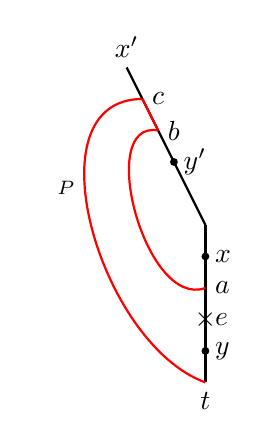
\begin{tikzpicture}[scale=2]
\begin{scope}
\coordinate (s) at (-0.5,2);
\coordinate (s1) at (0.5,2);
\coordinate (w) at (0,1);
\coordinate (t) at (0,0);
\coordinate (x) at (0,0.8);
\coordinate (y) at (0,0.2);
\coordinate (y1) at (-0.2,1.4);
\coordinate (i1) at (-0.4,1.8);
\coordinate (i2) at (-0.3,1.6);
\coordinate (a) at (0,0.6);
\coordinate (v) at (0,0.4);



\draw[thick](s)--(w);
%\draw[thick](s1)--(w);
\draw[thick](w)--(t);
\node[above] at (s){$x'$};
%\node[above] at (s1){$s$};
\node[below] at (t){$t$};

\node[right] at (a){$a$};

%\node[right] at (w){$w$};
\node[right] at (i1){$c$};
\node[right] at (i2){$b$};


\draw[red,thick] (a) to[out=200,in=170]
(i2);
\draw[red,thick](i1)--(i2);
\draw[red,thick] (i1) to[out=180,in=160]node[pos=0.4,left,black]{\scriptsize{$P$}}  (t);
\node at (v){$\times$};
\node[right] at (v){$e$};
\draw (y) node[fill,circle,scale=0.3]{};
\node[right] at (y){$y$};
\draw (x) node[fill,circle,scale=0.3]{};
\node[right] at (x){$x$};
\draw (y1) node[fill,circle,scale=0.3]{};
\node[right] at (y1){$y'$};
\end{scope}
\end{tikzpicture}
\caption{The path $P$ merges with another segment $x'y'$  and then diverges.}
\label{fig:feature}

\end{figure}

  \begin{proof}
  Once $P$ merges with $x'y'$ segment, it will diverge from it only if
  $x't$ contains $e$. This implies that $xt$ and $x't$ intersect or $xt$
  is a subpath of $x't$.
  %If $\DET(P)$ starts on $sw$ path
  %(before or on the intersection vertex $w$), then $P \in \TON$.
  %We will argue now that $\DET(P)$
  %cannot start after the intersection vertex.

  \noindent Assume for contradiction that $P \in \TTW$, that is, $\DET(P)$
  start strictly inside segment $xy$. Consider the Figure \ref{fig:feature} in which
  the detour of the preferred replacement path $P$
  starts after $x$ (at $a$). It then intersect  $x'y'$ at $b$
  and then diverges from $x't$ path at $c$.
  We claim that there exists another path to reach $b$ that is shorter  than
  $xa \conc ab$. This path is $xb$, where path $xb$ is a subpath of $x't$.
  It is also a shorter path (in $G_p$) as it uses
   edges in original $x't$ path.

  This path (1) diverges at $x$ and (2) is shorter (in $G_p$) as it uses edges from $x't$ path.
  Thus, there is a shorter replacement path than $P$ that avoids $e$. This path is not in
  $\TTW$ as its detour starts at $x$  .
  This leads to a contradiction as we had assumed that $P$ is the preferred replacement path avoiding $e$.
  Thus our assumption,
  namely that $P \in \TTW$ must be false.
  \end{proof}
\fi

\noindent We will now analyze  paths in $\TTW$. Consider two replacement
paths $P, P'$ avoiding edges $e,e'$ (respectively) on $xy,x'y'$ segment respectively.
%($ x,x'$  are intersection vertices in \SBFS($t$)) .
Let  $a,a'$ be the starting vertex of $\DET(P), \DET(P')$ respectively.
We say that $P \prec P'$ if $|at| < |a't|$.
If $|at| = |a't|$, then the tie is broken arbitrarily.


\noindent  Given a path $P \in \TTW$, let $(< P)$ be the set of all replacement
paths in $\TTW$ that are $\prec P$ in the ordering. Similarly, $(> P)$ is
the set of all replacement paths $P' \in \TTW$ for which $P \prec P'$.
Define $\UNQ(P)$ according to this ordering (see definition \ref{def:unique}).
Assume that we are processing a replacement path $P$ according to this ordering.
If $|\UNQ(P)| \ge \sqrt{n/\sigma}$, then we can associate $O(\sqrt{n/\sigma})$
{\em unique} vertices to $P$. Otherwise $|\UNQ(P)| < \sqrt{n/\sigma}$ and we have the following two cases:

\iflong
\else
\vspace{-2mm}
\fi



\subsection{ $\DET (P)$ does not intersect with any other detour in $(> P)$ }
\label{subsec:nointersect}
\noindent This case is similar to the first case in Section \ref{subsec:singlecaseone}.
\iflong
  Assume that $P$ avoids an edge $e$ on segment $xy$. Let $\DET(P)$
  start at $a \in xy$ and end at $b$ -- the vertex
  where it touches $t_xt$ path. Let $ab$ denote the
path from $a$ to $b$ on $P$. By our assumption $\UNQ(P)
  = ab$ and $|ab| < \sqrt{n/\sigma}$. Consider the following set
  of replacement paths  $(< P)_x := \{P' \in (< P)\ |\ P'~ \text{avoids an edge on $xy$ segment}\}$.
  By Lemma \ref{lem:avoids},
  all  replacement paths in $(< P)_x$ pass through $e$ (as
  detour of these replacement paths start below $e$) and by
  Lemma \ref{lem:avoidreverse}, these replacement paths avoid
  edges that are closer to $y$ than $e$. We can view these
  replacement paths as if they are starting from vertex $a$.
   $|P \setminus xa|
  = |ab| + |bt| \le \sqrt {n/\sigma} + |at|$. Using lemma \ref{lem:length}, total
  number of paths in   $(\le P)_x$ is  $\le \sqrt{ n/\sigma}$.  Thus, once we
  get a replacement path $P \in \TTW(xy)$ with $|\UNQ(P)| < \sqrt{n /\sigma}$, then there
  are at most $\sqrt{n/\sigma}$ replacement paths in $\TTW(xy)$ remaining to be processed.
  Thus, total number of paths in $\TTW$ with  $|\UNQ(P)|< \sqrt{n/\sigma}$ is
  $\sum_{xy \in \text{\SBFS($t$)}} \sqrt{n/ \sigma} = O(\sqrt{n \sigma})$
  (as there are $O(\sigma)$ segments in \SBFS($t$))
\else
   We can show that once we
   get a replacement path $P \in \TTW(xy)$ with $|\UNQ(P)| < \sqrt{n /\sigma}$, then there
   are at most $O(\sqrt{n/\sigma})$ replacement paths in $\TTW(xy)$ remaining to be processed. This will bound
   the total number of such paths to $O(\sqrt{n\sigma})$. Please see
   the full version for details.
\fi

\iflong
\else
\vspace{-2mm}
\fi
\subsection{ $\DET(P)$ intersects with  detour of a  path in $(> P)$}
\label{subsec:pintersects}

We first give a formal definition of a bad path that was defined informally in Section \ref{sec:problem}.
\begin{definition} (Bad Path)
A path $P \in \TTW$ is called a bad path if there exists another path $P' \in (>P)$
such that (1) $\DET(P)$ intersects with $\DET(P')$ and (2) $\DET(P')$ passes through the edge
avoided by $P$ after their intersection. We also say that $P$ is a bad replacement
path due to $P'$ if $P'$ satisfies the above two conditions.
\end{definition}

A path that is not bad is called a good path. In Section \ref{sec:problem}, we saw that
bad paths break the easy analysis of the single source case.
So, we have two cases depending on whether the path is good or bad. Let us look at the easier case first.\iflong\\\else\vspace{1mm}\fi


% Note that our analysis in Section \ref{sec:avoids} was easy as $P'$ cannot pass through $e$.
%However, as we have seen in Section \ref{sec:problem}, $P'$ can pass through $e$.
%Let us first look at the scenario when $P'$ does not pass through $e$ after intersection with $P$.
\iflong
\else
\section{SIMULATION RESULTS}
\label{sec:examples}
This section presents simulation results of the proposed method implemented on the unicycle model example.
Each semidefinite program was prepared using a custom software toolbox and the modeling tool YALMIP \cite{lofberg2004yalmip}.
The programs are run with commercial solver MOSEK on a machine with $1$ TB availabe memory. 

\subsection{FRS Computation}
We computed the FRS for a 3$^\text{rd}$ order Taylor-expanded Dubins car as the low-fidelity model $f_s$.
Trajectories produced by this model were tracked by the unicycle model from Equation \eqref{eq:big_dyn} as the high-fidelity model $f$.
The vehicle's representation as an initial distribution $X_0 \subset X_s$, was a rectangle of length $0.2$ [m] in $x$ and width $0.1$ [m] in $y$, at $0^\circ$ initial heading, and centered at $x=-0.75$ and $y=0$.
This is the same vehicle representation shown in all previous figures.

% The error function $g$, illustrated in Figure \ref{fig:error_dynamics}, was given by:
% \begin{equation}
% \label{eq:g_definition}
% g(t,x_s) = \begin{bmatrix}
% v_\text{err}\cdot(1 - \frac{1}{2}\theta^2)  \\
% v_\text{err}\cdot(\theta - \frac{1}{6}\theta^3) \\
% \dot{\theta}_\text{err}
% \end{bmatrix}
% \end{equation}
% where $v_\text{err} = (t-1)^2$ and $\dot{\theta}_\text{err} = (t-1)^4$.
We chose $\tau_\text{stop} = \tau_\text{plan} = 0.5$ [s], so $T = 1$ [s].
The stopping time can be seen in Figure \ref{fig:error_dynamics}. 
The FRS computation took 79 hours and used a maximum of 150 GB of memory 
%on a server with 1 TB of available memory and 18 processors each running at 1.2 GHz.

\subsection{Set Intersection and Trajectory Planning}

We used the precomputed FRS for safe trajectory planning in $1000$ simulated trials in MATLAB on the aforementioned machine.
For each trial, the vehicle began at the same initial location and heading, surrounded by $1-10$ randomized obstacles and a randomly-located goal to reach.
%If the planning time took more than $\tau_\text{plan}$, the simulation paused until the computation was complete. 
%In practice, if $\tau_\text{plan}$ was exceeded the vehicle could begin braking to ensure safety.
The vehicle's initial speed, and the desired speed to maintain for the duration of the trial, were randomly chosen between $0.25$ and $0.75$ [m/s].
% The trials ran in 12.7 hours.
% Prior to running these trials, several example trials were run on a laptop with a 2.3 GHz processor and 16 GB of RAM.
% The trials run on the server were individually no faster than running on the laptop, because the set intersection optimization is a single-core process that uses very little memory. 
% Therefore, the server did not provide any significant decrease in the implemented planning time.


Obstacles were represented as line segments between $0.1$ and $0.2$[m] in length, with random location and orientation.
The obstacles were always placed between the vehicle and the goal.
We checked for crashes conservatively for each trial, by inspecting if any obstacle was within a circle circumscribing the rectangular vehicle at any point of the vehicle's trajectory. 
Using this method, \emph{no crashes were detected in any trial}.
Out of all the trials, $82\%$ reached the goal, and $15\%$ performed an emergency braking maneuver (by setting $v_\text{des} = 0$). 
The remaining 3\% hit a simulation iteration limit.
Examples of the vehicle's path from a randomly-generated trial and from two constructed emergency braking cases are shown in Figure \ref{fig:example_trial}.


\begin{figure}
\centering
\includegraphics[width=1\columnwidth]{running_examples.pdf}
\caption{The top subplot shows an example result out of the $1000$ trials.
This trial used eight randomly-generated obstacles.
The vehicle begins on the left at $x = -0.75$ and reaches a randomly-generated goal near $(2.5, 0.5)$, plotted as a blue circle.
Every $\tau_\text{plan} = 0.5$[s], the vehicle replans its trajectory, shown by an asterisk plotted on the global trajectory in blue.
The bounding box of the vehicle at each planning step is shown as a grey rectangle. In the bottom-left subplot, an obstacle was constructed between the vehicle and the goal, forcing an emergency braking maneuver. In the bottom-right subplot, an obstacle was constructed with a hole that would allow the vehicle to pass, but the set intersection result is overly conservative, resulting in a braking maneuver.}
\label{fig:example_trial}
\end{figure}

Currently, our implementation cannot consistently achieve $\tau_\text{plan} = 0.5$ [s].
Consequently, instead of replanning and driving simultaneously, we pause time every 0.5 [s] of the simulation to guarantee that the vehicle can finish replanning.
In a physical implementation, if $\tau_\text{plan}$ is exceeded, then the vehicle must emergency brake; recall that a safe braking trajectory is always available.
As shown in Figure \ref{fig:planning_time_vs_Nobs}, $\tau_\text{plan}$ scales linearly with the number of obstacles.
%Methods for reducing the set intersection to meet $\tau_\text{plan}$ will be presented in future work.

\begin{figure}
\centering
\includegraphics[scale=0.45,trim={1cm 6cm 1cm 7cm},clip]{planning_time_vs_Nobs.pdf}
\caption{The mean set intersection time (top) and trajectory optimization time (bottom) versus the number of obstacles. Over the $1000$ trials, each number of obstacles from $1$ to $10$ was used for $100$ trials. Notice that set intersection takes up to $3$[s], and scales with the number of obstacles. On the other hand, the trajectory optimization takes around $80$ [ms] and has low correlation with number of obstacles.}
\label{fig:planning_time_vs_Nobs}
\end{figure}

% \begin{figure}
% \centering
% \includegraphics[scale=0.5,trim={1cm 8cm 1cm 8cm},clip]{example_trial_bluecar.pdf}
% \caption{An example result out of the 1000 trials.
% This trial used eight randomly-generated obstacles.
% The vehicle begins on the left at $x = -0.75$ and reaches a randomly-generated goal near $(2.5, 0.5)$, plotted as a blue circle.
% Every $\tau_\text{plan} = 0.5$ [s], the vehicle replans its trajectory, shown by an asterisk plotted on the global trajectory in blue.
% The bounding box of the vehicle at each planning step is shown as a grey rectangle.}
% \label{fig:example_trial}
% \end{figure}

% \begin{figure}
% \centering
% \includegraphics[scale=0.4,trim={1cm 7cm 1cm 7cm},clip]{example_emergency_brake.pdf}
% \caption{An example of a forced emergency braking situation. The vehicle cannot find a path to the desired location (plotted as a blue circle), so it brakes.}
% \label{fig:example_emergency_brake}
% \end{figure}

% \begin{figure}
% \centering
% \includegraphics[scale=0.4,trim={1cm 7cm 1cm 7cm},clip]{example_overly_conservative.pdf}
% \caption{An example of an unnecessary emergency braking situation. The vehicle cannot find a path to the desired location despite an obviously-safe path existing, because the FRS is overly conservative.}
% \label{fig:example_overly_conservative}
% \end{figure}

\fi
\iflong\section{SIMULATION RESULTS}
\label{sec:examples}
This section presents simulation results of the proposed method implemented on the unicycle model example.
Each semidefinite program was prepared using a custom software toolbox and the modeling tool YALMIP \cite{lofberg2004yalmip}.
The programs are run with commercial solver MOSEK on a machine with $1$ TB availabe memory. 

\subsection{FRS Computation}
We computed the FRS for a 3$^\text{rd}$ order Taylor-expanded Dubins car as the low-fidelity model $f_s$.
Trajectories produced by this model were tracked by the unicycle model from Equation \eqref{eq:big_dyn} as the high-fidelity model $f$.
The vehicle's representation as an initial distribution $X_0 \subset X_s$, was a rectangle of length $0.2$ [m] in $x$ and width $0.1$ [m] in $y$, at $0^\circ$ initial heading, and centered at $x=-0.75$ and $y=0$.
This is the same vehicle representation shown in all previous figures.

% The error function $g$, illustrated in Figure \ref{fig:error_dynamics}, was given by:
% \begin{equation}
% \label{eq:g_definition}
% g(t,x_s) = \begin{bmatrix}
% v_\text{err}\cdot(1 - \frac{1}{2}\theta^2)  \\
% v_\text{err}\cdot(\theta - \frac{1}{6}\theta^3) \\
% \dot{\theta}_\text{err}
% \end{bmatrix}
% \end{equation}
% where $v_\text{err} = (t-1)^2$ and $\dot{\theta}_\text{err} = (t-1)^4$.
We chose $\tau_\text{stop} = \tau_\text{plan} = 0.5$ [s], so $T = 1$ [s].
The stopping time can be seen in Figure \ref{fig:error_dynamics}. 
The FRS computation took 79 hours and used a maximum of 150 GB of memory 
%on a server with 1 TB of available memory and 18 processors each running at 1.2 GHz.

\subsection{Set Intersection and Trajectory Planning}

We used the precomputed FRS for safe trajectory planning in $1000$ simulated trials in MATLAB on the aforementioned machine.
For each trial, the vehicle began at the same initial location and heading, surrounded by $1-10$ randomized obstacles and a randomly-located goal to reach.
%If the planning time took more than $\tau_\text{plan}$, the simulation paused until the computation was complete. 
%In practice, if $\tau_\text{plan}$ was exceeded the vehicle could begin braking to ensure safety.
The vehicle's initial speed, and the desired speed to maintain for the duration of the trial, were randomly chosen between $0.25$ and $0.75$ [m/s].
% The trials ran in 12.7 hours.
% Prior to running these trials, several example trials were run on a laptop with a 2.3 GHz processor and 16 GB of RAM.
% The trials run on the server were individually no faster than running on the laptop, because the set intersection optimization is a single-core process that uses very little memory. 
% Therefore, the server did not provide any significant decrease in the implemented planning time.


Obstacles were represented as line segments between $0.1$ and $0.2$[m] in length, with random location and orientation.
The obstacles were always placed between the vehicle and the goal.
We checked for crashes conservatively for each trial, by inspecting if any obstacle was within a circle circumscribing the rectangular vehicle at any point of the vehicle's trajectory. 
Using this method, \emph{no crashes were detected in any trial}.
Out of all the trials, $82\%$ reached the goal, and $15\%$ performed an emergency braking maneuver (by setting $v_\text{des} = 0$). 
The remaining 3\% hit a simulation iteration limit.
Examples of the vehicle's path from a randomly-generated trial and from two constructed emergency braking cases are shown in Figure \ref{fig:example_trial}.


\begin{figure}
\centering
\includegraphics[width=1\columnwidth]{running_examples.pdf}
\caption{The top subplot shows an example result out of the $1000$ trials.
This trial used eight randomly-generated obstacles.
The vehicle begins on the left at $x = -0.75$ and reaches a randomly-generated goal near $(2.5, 0.5)$, plotted as a blue circle.
Every $\tau_\text{plan} = 0.5$[s], the vehicle replans its trajectory, shown by an asterisk plotted on the global trajectory in blue.
The bounding box of the vehicle at each planning step is shown as a grey rectangle. In the bottom-left subplot, an obstacle was constructed between the vehicle and the goal, forcing an emergency braking maneuver. In the bottom-right subplot, an obstacle was constructed with a hole that would allow the vehicle to pass, but the set intersection result is overly conservative, resulting in a braking maneuver.}
\label{fig:example_trial}
\end{figure}

Currently, our implementation cannot consistently achieve $\tau_\text{plan} = 0.5$ [s].
Consequently, instead of replanning and driving simultaneously, we pause time every 0.5 [s] of the simulation to guarantee that the vehicle can finish replanning.
In a physical implementation, if $\tau_\text{plan}$ is exceeded, then the vehicle must emergency brake; recall that a safe braking trajectory is always available.
As shown in Figure \ref{fig:planning_time_vs_Nobs}, $\tau_\text{plan}$ scales linearly with the number of obstacles.
%Methods for reducing the set intersection to meet $\tau_\text{plan}$ will be presented in future work.

\begin{figure}
\centering
\includegraphics[scale=0.45,trim={1cm 6cm 1cm 7cm},clip]{planning_time_vs_Nobs.pdf}
\caption{The mean set intersection time (top) and trajectory optimization time (bottom) versus the number of obstacles. Over the $1000$ trials, each number of obstacles from $1$ to $10$ was used for $100$ trials. Notice that set intersection takes up to $3$[s], and scales with the number of obstacles. On the other hand, the trajectory optimization takes around $80$ [ms] and has low correlation with number of obstacles.}
\label{fig:planning_time_vs_Nobs}
\end{figure}

% \begin{figure}
% \centering
% \includegraphics[scale=0.5,trim={1cm 8cm 1cm 8cm},clip]{example_trial_bluecar.pdf}
% \caption{An example result out of the 1000 trials.
% This trial used eight randomly-generated obstacles.
% The vehicle begins on the left at $x = -0.75$ and reaches a randomly-generated goal near $(2.5, 0.5)$, plotted as a blue circle.
% Every $\tau_\text{plan} = 0.5$ [s], the vehicle replans its trajectory, shown by an asterisk plotted on the global trajectory in blue.
% The bounding box of the vehicle at each planning step is shown as a grey rectangle.}
% \label{fig:example_trial}
% \end{figure}

% \begin{figure}
% \centering
% \includegraphics[scale=0.4,trim={1cm 7cm 1cm 7cm},clip]{example_emergency_brake.pdf}
% \caption{An example of a forced emergency braking situation. The vehicle cannot find a path to the desired location (plotted as a blue circle), so it brakes.}
% \label{fig:example_emergency_brake}
% \end{figure}

% \begin{figure}
% \centering
% \includegraphics[scale=0.4,trim={1cm 7cm 1cm 7cm},clip]{example_overly_conservative.pdf}
% \caption{An example of an unnecessary emergency braking situation. The vehicle cannot find a path to the desired location despite an obviously-safe path existing, because the FRS is overly conservative.}
% \label{fig:example_overly_conservative}
% \end{figure}
\fi

\noindent {(1) \em $P$ is a good path.}

\noindent Assume that $P \in \TTW(xy)$ and it avoids an edge $e \in xy$.
Assume that $P$  intersects first with $P' \in (> P)$ and $P'$ avoids $e'$ on $x'y'$ segment.
Note that $x$ may be equal to $x'$.
Let $\DET(P')$ start at $a'$ and end at
$b'$. Assume that $\DET(P)$ starts at $a$ and it intersects $\DET(P')$
at $c$.
Consider the path $x'a' \conc a'c \conc ca \conc at$. Since $x'a' \conc a'c$ is a part of $P'$,
it avoids $e'$. However, it is not clear whether $ca \conc at$ avoids $e'$ too.
In Figure \ref{fig:examples}, we see two representative examples in which $ca$ and $at$
avoid $e'$.
\iflong
  We will now show that both $ca$   and $at$ cannot passes through $e'$.
  %then $P$ is {\em similar} to $P'$
  %(in which case we can discard path $P$).
  \begin{enumerate}
   \item[(a)] Assume that  $ca$ passes through $e'$ %(See Figure \ref{fig:badexample1}(a))
    \label{enum:goodcase}

  If $x=x'$, then by Lemma \ref{lem:avoids}, as $P' \in (>P)$, $\DET(P)$ (and hence $ca$)
   starts below $e'$. Thus, $ca$ cannot pass through $e'$ as $\DET(P)$ does not
  intersect $xt_x$ path and $e' \in xt_x$. So let us assume that $x \neq x'$.
  This implies that $P$ intersects $x'y'$. After intersecting $x'y'$ path
    $P$ did not follow $x'y' \conc y't$ (since $ca$ intersect $\DET(P')$ at $c$).
    %This implies that $s't$ path contains $e$ (the vertex $P$ avoids).
    %Thus, $s't$ and $st$ intersect, say at $w$ and $e$ lies after $w$ on $s't$
    %and $st$ path. Since $P \in \TTW$, $\DET(P)$ should also start after $w$.
    %Since $\DET(P)$ passes through $e'$, $e'$ cannot lie on $wt$ path
    %(as $wt$ is a subpath of $st$ and by defintion $\DET(P)$ cannot intersect $st$).
    %Thus $e' \in sw$.
    This implies that $P$ intersect with another path $x'y'$ and then
    diverges. By Lemma \ref{lem:feature}, $P \notin \TTW$.
    This leads to a contradiction as we assumed that $P \in \TTW$. Thus our
    assumption, namely $ca$ passes through
    $e'$ is false.


    %Now, we have to satisfy two conditions (1) $\DET(P)$ should start below $w$ and (2) $\DET(P)$ should pass through $w$.  We claim that $P$ cannot satisfy both the condition. This is because the best vertex for a detour to start to satisfy condition (2) is $w$, the intersection vertex of $s't$ and $st$.


    %Thus, such a $P$ cannot exists as we have reached a contradiction. So, $ca$ cannot pass through $e'$.

  \item[(b)] Assume that $at$ passes through $e'$ %(See Figure \ref{fig:badexample1}(b))
  \label{enum:one}

  If $x = x'$, then by Lemma \ref{lem:avoids}, starting vertex of $\DET(P)$, that is $a$, starts below $e'$. Thus,
  $at$ cannot pass through $e'$. So let us assume that $x \neq x'$.
  If $at$ passes through $e'$, then segment $x'y'$ is a subpath of $xt$ path.
  This is due to the fact that $a \in xy$ and $e' \in x'y'$. Since $P' \in \TTW(x'y')$,
  $\DET(P')$ starts strictly inside segment $x'y'$, at vertex $a'$. This implies that $|a't| < |at|$.
  This contradicts our assumption that $P' \in (>P)$. Thus, $at$ cannot pass through $e'$.
  %Once again $x \neq x'$
  %Since $a \in st$ and $e' \in s't$, this implies that $st$ and $s't$ intersect at $w$
  %and $e'$ lies in $wt$ path.
  %Since $P' \in \TTW$, $\DET(P')$ should also
  %start in $wt$.  Since $P' \in (>P)$, $|a't| \ge |at|$. We claim that $a't$
  %contains both $e$ and $e'$. This is due to the fact that $e \in at$, $|a't| \ge |at|$
  %and by assumption $e' \in at$.
  %Thus we have two path $P$ and $P'$ that are meet at vertex $w$ after which
  %their detour start at $a$ and $a'$ respectively and  both these detours
  %avoid $e'$ and $e$. So, the preferred path avoiding $e$ and $e'$ from $w$ is either the suffix of $P$ or $P'$ -- the one which is the shortest replacement path and leaves $wt$ path as early as possible.
  %This implies that both $P$ and $P'$ have same detour
  %and they start from the same vertex, that is $a = a'$.



  %We claim that $e$ cannot lie on $wt$ path as it then leads
  %to case \ref{}, which is known to be an easy scenario. This implies that $|at| > |a't|$. Thus, $P' \notin (>P)$. This leads to a contradiction as we started out with the assumption that $P' \in (>P)$.

  \end{enumerate}
\fi


%When viewed from the vantage point of intersection vertex
%$w$,
%there is no difference between $P$ and $P'$. Thus, we discard
%$P$.

%Thus, if $P$ is not discarded, then both $ca$ and $at$ also avoid $e'$.
\iflong\else In the full version of the paper, we show that $ca$ and $at$ cannot pass through $e'$. \fi
Thus, the path $x'a' \conc a'c \conc ca \conc at$ is indeed a valid replacement
path from $x'$ to $t$ avoiding $e'$. Since $P' = x'a' \conc a'c \conc cb' \conc b't$, length
of $P'$ must be $\le$ length of  this alternate path. Thus,\\
\begin{tabular}{llll}
& $|x'a'| +  |a'c|
+ |cb'| + |b't|$& $\le$ & $|x'a'| + |a'c| + |ca|  + |at|$  \\
$\implies$& $
|cb'| + |b't|$ & $\le$ & $|ca|  + |at|$   \\
$\implies$&$|ac| +
|cb'| + |b't|$ & $\le$ &  $2|ca|  + |at|$

\end{tabular}
%\begin{figure}
\centering
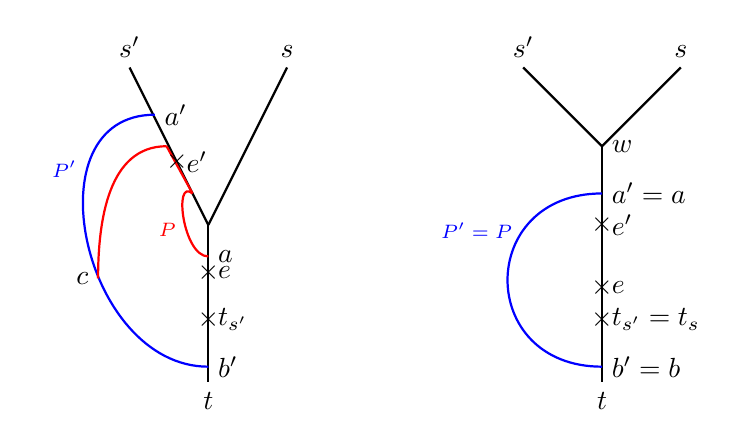
\begin{tikzpicture}[scale=2]
\begin{scope}
\coordinate (s) at (-0.5,2);
\coordinate (s1) at (0.5,2);
\coordinate (w) at (0,1);
\coordinate (t) at (0,0);
\coordinate (ts) at (0,0.4);
\coordinate (b1) at (0,0.1);

\coordinate (i1) at (-0.265,1.5);
\coordinate (i2) at (-0.1,1.2);

\coordinate (a1) at (-0.34,1.7);
\coordinate (a) at (0,0.8);
\coordinate (v) at (0,0.7);
\coordinate (v1) at (-0.2,1.4);
\coordinate (c) at (-0.7,0.66);

\draw[thick](s)--(w);
\draw[thick](s1)--(w);
\draw[thick](w)--(t);
\node[above] at (s){$s'$};
\node[above] at (s1){$s$};
\node[below] at (t){$t$};
\node[right] at (a1){$a'$};
\node[right] at (a){$a$};
\node[right] at (b1){$b'$};
\node[left] at (c){$c$};


\draw[blue,thick] (a1) to[out=180,in=180,distance=.8cm]
node[pos=0.3,left]
{\scriptsize  $P'$}  (b1);

\draw[red,thick] (a) to[out=180,in=140]
node[pos=0.4,left]
{\scriptsize  $P$}  (i2);
\draw[red,thick](i1)--(i2);
\draw[red,thick] (i1) to[out=180,in=90](c);

\node at (v1){$\times$};
\node[right] at (v1){$e'$};

\node at (v){$\times$};
\node[right] at (v){$e$};

\node at (ts){$\times$};
\node[right] at (ts){$t_{s'}$};

\end{scope}
\begin{scope}[xshift=2.5cm]
\coordinate (s) at (-0.5,2);
\coordinate (s1) at (0.5,2);
\coordinate (w) at (0,1.5);
\coordinate (t) at (0,0);
\coordinate (ts) at (0,0.4);
\coordinate (b1) at (0,0.1);

\coordinate (i1) at (-0.265,1.5);
\coordinate (i2) at (-0.1,1.2);

\coordinate (a1) at (0,1.2);
\coordinate (a) at (0.29,1.6);
\coordinate (v) at (0,0.6);
\coordinate (v1) at (0,1);
\coordinate (c) at (-0.7,0.66);

\draw[thick](s)--(w);
\draw[thick](s1)--(w);
\draw[thick](w)--(t);
\node[above] at (s){$s'$};
\node[above] at (s1){$s$};
\node[below] at (t){$t$};
\node[right] at (a1){$a'=a$};
\node[right] at (w){$w$};
\node[right] at (b1){$b'=b$};



\draw[blue,thick] (a1) to[out=180,in=180,distance=.8cm]
node[pos=0.3,left]
{\scriptsize  $P'=P$}  (b1);


\node at (v1){$\times$};
\node[right] at (v1){$e'$};

\node at (v){$\times$};
\node[right] at (v){$e$};

\node at (ts){$\times$};
\node[right] at (ts){$t_{s'} = t_s$};

\end{scope}
\end{tikzpicture}
\caption{ffs}
\label{fig:badexample1}

\end{figure}


On the left hand of the inequality, we  have a path from
$a$ to $t$ avoiding $e$ (since we know that $P$ is a good path, so $P'$ and thus $cb' \conc b't$ does not
pass through $e$). So, its length should be $\ge$
length of the preferred path $P \setminus xa$. Thus $|P
\setminus xa| \le 2|ca|  + |at| \le 2\sqrt {n/\sigma}\
+\ |at|$ (since $|\UNQ(P)| = |ac| < \sqrt{n/\sigma}$). Consider the following set of replacement paths  $(< P)_x
:= \{P' \in (< P)\ |\ P' \ \text{avoids
an edge on $xy$ segment}\}$. By Lemma \ref{lem:avoids},
all  replacement paths in $(<P)_x$ pass through $e$ (as
detour of these replacement paths start below $e$) and by
Lemma \ref{lem:avoidreverse}, these replacement paths avoid
edges that are closer to $y$ than $e$.
  Applying Lemma \ref{lem:length}, we get
that  the number of replacement paths $(<P)_x$  is $ \le 2\sqrt{n/\sigma}$. Thus, once we
get a replacement path $P \in \TTW(xy)$ with $|\UNQ(P)| < \sqrt{n /\sigma}$, then there
are at most $2\sqrt{n/\sigma}$ replacement paths in $\TTW(xy)$ remaining to be processed.
Thus, total number of paths $\in \TTW$ with  $|\UNQ(P)| < \sqrt{n/\sigma}$ is
$\sum_{xy \in \text{\SBFS($t$)}} 2\sqrt{n/\sigma} = O(\sqrt{n \sigma})$
(as there are $O(\sigma)$ segments in \SBFS($t$)).\iflong\\\else\vspace{2mm}\fi

\iflong
   \begin{figure}[hpt!]
\centering
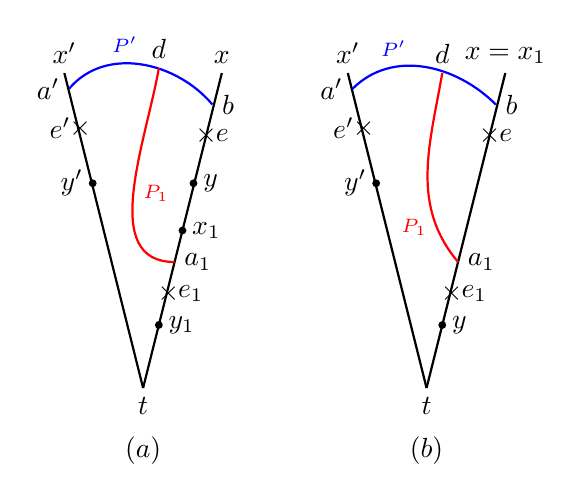
\begin{tikzpicture}[scale=2]
\begin{scope}
\coordinate (s) at (0.5,2);
\coordinate (s1) at (-0.5,2);
%\coordinate (s2) at (1.1,2);
%\coordinate (w) at (0.5,1.4);
\coordinate (t) at (0,0);
\coordinate (ts) at (0.15,0.4);
\coordinate (b) at (0.44,1.8);
\coordinate (y1) at (-0.32,1.3);
\coordinate (y) at (0.32,1.3);

\coordinate (x2) at (0.25,1);
\coordinate (y2) at (0.1,0.4);

\coordinate (a1) at (-0.47,1.9);
\coordinate (a2) at (0.2,0.8);
\coordinate (v) at (0.4,1.6);
\coordinate (v1) at (-0.4,1.65);
\coordinate (v2) at (0.16,0.6);
\coordinate (c) at (-0.7,0.66);
\coordinate (d) at (0.1,2.03);

\draw[thick](s)--(t);
\draw[thick](s1)--(t);
%\draw[thick](s2)--(w);
%\draw[thick](w)--(t);
\node[above] at (s){$x$};
\node[above] at (s1){$x'$};
%\node[above] at (s2){$s_1$};
\node[below] at (t){$t$};
\node[left] at (a1){$a'$};
\node[right] at (b){$b$};

\node[above] at (d){$d$};
%\node[right] at (w){$w$};


\draw[blue,thick] (a1) to[out=50,in=130]
node[pos=0.4,above]
{\scriptsize  $P'$}  (b);



\draw[red,thick] (a2) to[out=180,in=260]
node[pos=0.5,right]
{\scriptsize  $P_1$}  (d);

\node at (v1){$\times$};
\node[left] at (v1){$e'$};


\node[right] at (a2){$a_1$};

\node at (v){$\times$};
\node[right] at (v){$e$};

\node at (v2){$\times$};
\node[right] at (v2){$e_1$};

%\node at (ts){$\times$};
%\node[right] at (ts){$t_{s}$};

\draw (y1) node[fill,circle,scale=0.3]{};
\node[left] at (y1){$y'$};

\draw (y) node[fill,circle,scale=0.3]{};
\node[right] at (y){$y$};

\draw (x2) node[fill,circle,scale=0.3]{};
\node[right] at (x2){$x_1$};

\draw (y2) node[fill,circle,scale=0.3]{};
\node[right] at (y2){$y_1$};

\node at (0,-0.4){$(a)$};

\end{scope}
\begin{scope}[xshift=1.8cm]
\coordinate (s) at (-0.5,2);
\coordinate (s1) at (0.5,2);

\coordinate (t) at (0,0);
\coordinate (ts) at (0.1,0.4);
\coordinate (b) at (0.44,1.8);

\coordinate (a2) at (0.2,0.8);
\coordinate (d) at (0.1,2);
\coordinate (y1) at (-0.32,1.3);
\coordinate (y) at (0.1,0.4);
\coordinate (a1) at (-0.47,1.9);
\coordinate (a) at (0.1,0.8);
\coordinate (v) at (0.4,1.6);
\coordinate (v2) at (0.16,0.6);
\coordinate (v1) at (-0.4,1.65);
\coordinate (c) at (-0.7,0.66);

\draw[thick](s)--(t);
\draw[thick](s1)--(t);

\node[above] at (s){$x'$};
\node[above] at (s1){$x=x_1$};
\node[below] at (t){$t$};
\node[left] at (a1){$a'$};

\node[right] at (b){$b$};
\node[right] at (a2){$a_1$};
\node[above] at (d){$d$};

\draw[blue,thick] (a1) to[out=45,in=135]
node[pos=0.3,above]
{\scriptsize  $P'$}  (b);


\draw[red,thick] (a2) to[out=130,in=260]
node[pos=0.2,left]
{\scriptsize  $P_1$}  (d);

\node at (v1){$\times$};
\node[left] at (v1){$e'$};

\node at (v2){$\times$};
\node[right] at (v2){$e_1$};

\node at (v){$\times$};
\node[right] at (v){$e$};



\draw (y1) node[fill,circle,scale=0.3]{};
\node[left] at (y1){$y'$};

\draw (y) node[fill,circle,scale=0.3]{};
\node[right] at (y){$y$};

\node at (0,-0.4){$(b)$};
\end{scope}
\end{tikzpicture}
\caption{Two cases in which $P'$ passes through $e_1$ after intersecting with $P_1$}
\label{fig:badexample}

\end{figure}

\fi
\noindent  {(2) \em $P$ is a bad path.}
\label{enum:two}

\noindent We now arrive at our hardest scenario.
We will first show that the number of good paths in $\TTW$
is greater than
the number of bad paths in $\TTW$.
To this end, we will prove the following lemma:
\begin{lemma}
\label{lem:badpaths}
For each $P' \in \TTW$, there exists only one replacement
path $P \in \TTW$ which is bad
due to $P'$.
\end{lemma}

\iflong
  \begin{proof}

  Assume that $P$ is the preferred path
  from $x$ to $t$ avoiding $e$ on segment $xy$. Similarly, $P'$ is the preferred path from $x'$ to $t$ avoiding $e'$ on segment $x'y'$ and $P$ is bad due to $P'$. Assume for contradiction that there is one more replacement
  path $P_1$ which is bad
  due to $P'$.
  %, that is,  1)$P_1 \in \TTW \cap (<P')$ and
  %$\DET(P_1)$ intersects with $\DET(P')$ and
  %(2) $\DET(P')$ passes through the edge avoided by $P_1$
  %after their intersection.
  Let us assume that $P_1$ avoids $e_1$ on $x_1y_1$ segment.
  If $x' = x$ or $ x'= x_1$, then $\DET(P')$ cannot pass through
  $e$ or $e_1$ respectively as
  $\DET(P')$ starts before $e$ or $e_{1}$ (as $P' \in (>P)$ or $P' \in (>P_1)$) and touches $x't$ path only at $t_{x'}t$. So, let us assume
  that $x' \neq x$ and $ x' \neq x_1$.

  Since $P' \in \TTW$, by lemma \ref{lem:feature}, we know
  that it follows $xt$ path after hitting segment $xy$, say at $b$. This
  implies
  that $e_1$ also lies on the $xt$ path. Thus, $xt$ and $x_1t$
  intersect. Without loss of generality, assume that  the segment $x_1y_1$ is
  a subpath of $xt$.
  %, say at $w$.
  %Assume without loss of generality
  %that $v_1$ is closer to $t$ than $v$ on $st$ path
  %\begin{enumerate}
  %   \item   $s_1 = s$
  %Note that if $x=x_1$, then $w := x=sx_1$.
  %Without loss of generality assume that $e_1$ is closer to
  %$t$ than $e$. %or $e_1=e$.
  %We have assumed that $P'$ passes through $e$.
  %By Lemma \ref{lem:feature},
  %we know that since $P' \in \TTW$, once it  hits $st$ path
  %(say at $b)$,
  %it cannot leave it.
  %By Lemma \ref{lem:avoids}, $\DET(P_1)$ starts below $v$
  %on $st$ path.
  Let us assume that $\DET(P_1)$ starts at $a_1$ and it
  hits $P'$ at $d$.
  There are two ways for $P_1$ to reach $d$ (both avoiding
  $e_1$):
  $x_1a_1 \conc a_1d$ and $x_1b \conc bd$
  where the first path is using the detour of $P_1$ and the second path
  uses $xt$ path to reach $b$.

  Note that the second path leaves the $x_1t$ path earlier than the
  first path ($x_1$ compared to $a_1$ if $x \neq x_1$ (Figure  \ref{fig:badexample}(a)) and
  $b$ compared to $a_1$ if $x=x_1$ (Figure  \ref{fig:badexample}(a))). Even then the preferred
  path used the first alternative.
  This implies that the length of the first path
  must be {\em strictly} less than the second.  Thus,
  $|x_1a_1| + |a_1d| < |x_1b| + |bd|$. Thus,
  \begin{equation}
  |a_1d| < |db| + |bx_1| - |x_1a_1|
  \end{equation}
  $P'$ takes the following path
  $x'a' \conc a'b \conc bt$.
  But there is  an alternative path available for $P'$, it
  is $x'a' \conc a'd \conc da_1 \conc a_1t$.
  The path is a valid path avoiding $e'$ only if $a_1d$
  does not pass through $e'$. All other components of this
  path are a part of $P'$ ($a'd \in a'b$ and $a_1t \in bt$)
  .

  If $a_1d$ does not pass through $e'$, then we can show that
  the alternative path has a length less than $|P'|$, thus arriving
  at a contradiction.
  Consider the length of the alternative path:
  \begin{tabbing}
   $|x'a'| $\=$+ |a'd| + |da_1| + |a_1t|$\\
   \>$< |x'a'|+ |a'd| + |db|  + |bx_1| - |x_1a_1| + |a_1t|$
  \hspace{10mm}\ (Using  Equation (1))\\\\
  If $x \neq x'$(See Figure  \ref{fig:badexample}(a)), then
  $ |bx_1|  - |x_1a_1|
  + |a_1t| \le  |bx_1|  + |x_1a_1| + |a_1t| = |bt|$. Else if $x
  =x'$ \\
  (See Figure  \ref{fig:badexample}(b)), then $ |bx_1|  - |x_1a_1|
  + |a_1t| = -|ba_1| +\ |a_1t| \le|ba_1| +\ |a_1t| =  |bt|$ \\\\
   \>$\le |x'a'|+ |a'd| + |db| + |bt|$\\
  \>$= |x'a'|+ |a'b| + |bt|$\\
   \>$= |P'|$
  \end{tabbing}

  This leads to a contradiction as we have assumed that $P'$
  is
  the shortest path from $x'$ to $t$ avoiding $e'$.

  To end this proof, we will show that $a_1d$ cannot pass
  through $e'$.
  Assume for contradiction that $a_1d$ passes through $e'$.
  This
  implies that $\DET(P_1)$ intersects with $x'y'$ segment (as
  $e' \in x'y'$) and
  then diverges from it (as $\DET(P_1)$ intersect with $\DET(P')$
  at $d$).
  By Lemma \ref{lem:feature}, $P_1 \notin \TTW$. But this cannot
  be the
  case as we have assumed that $P_1 \in  \TTW$. Thus our assumption,
  namely $a_1d$ passes through $e'$ must be false.


  %\item $s''=s$

  %Assume without loss of generality \todo{Is this wlog fine}
  %that $e''$ lies below $e$ on $st$ path. By Lemma \ref{},
  %we know that $P'$ leaves $st$ above $e$ and merges back
  %only at $t_st$ path. Since $e' \notin t_st$, this implies
  %that $P'$ can never pass through $e'$. Thus, we arrive
  %at a contradiction.

  %\item $s_1 \neq s$

  %Since $P' \in \TTW$, by lemma \ref{lem:feature}, we know
  %that it follows $st$ path after hitting it. This implies
  %that $v_1$ also lies on the $st$ path. Thus, $st$ and $s_1t$
  %intersect, say at $w$. Assume without loss of generality
  %that $v_1$ is closer to $t$ than $v$ on $st$ path. So,
  %$P_1$ satisfies two condition: (1) It intersects with $P'$
  %and (2) The vertex avoided by $P'$ is closer to $s$ than
  %$v''$. By Lemma \ref{}, we infer than $P'' \in \TON$. Thus,
  %we again arrive at a contradiction.

  %\end{enumerate}
  \end{proof}
\fi




%We now put the above lemma to use. We use the following
%algorithm to weed out paths that satisfy case 1(b) and case
%2.

%\begin{algorithm}
%\ForEach{$P \in \TTW$ precessed according to the ordering
%$\prec$}
%{
%    $\BP \leftarrow \emptyset$; \tcp{Set of Bad Paths}

%    $\GP \leftarrow \emptyset$; \tcp{Set of Good Paths}

%    \If{$\exists$ \ \text{a path in $GP$ whose detour start
%at the same vertex as of $P$\ }}
%    {
%        continue;
%    }
%    \If{ $\exists P' \in \GP$ such that $P'$ passes through
%$e$ after intersecting $P$ }
%    {

%        $\BP \leftarrow \BP \cup  \{P\}$\;
    % }
%     \Else
%     {
%         $\GP \leftarrow \GP \cup \{P\}$\;
%     }
% }
% \end{algorithm}

% The above algorithm discards a path $P$ if there already
% exists a processed good path whose detour starts from the
% same vertex as that of $P$. This takes care of case \ref{enum:one}.
% It then removes all the replacement paths $P$ that satisfy
% the conditions in Case \ref{enum:two}. $\BP$ is the set
% of paths removed by the algorithm. For each such path, there
% exists a path $P' \in \GP$. By Lemma \ref{lem:badpaths},
% we know that each good path in $\GP$ can remove atmost one
% bad path. This implies that the number of bad paths removed
% is $\le$ number of good paths, that is $|\BP| \le |\GP|$.
% All the paths in $\GP$ do not satisfy case \ref{enum:one}
% and \ref{enum:two}. Thus, these paths satisfy  case \ref{enum:goodcase}.

The above lemma can be used to discard bad paths from $\TTW$.
For each such discarded path, there exists at least one good path.
And by the above lemma, each such good path can be used to discard
at most one bad path. Thus the number of good paths in $\TTW$
is $\ge$ number of bad paths in $\TTW$.
We have already shown that the total number of good paths in $\TTW$
is $O(\sqrt{n\sigma})$.
Thus the total number of paths in $\TTW$ is also $O(\sqrt{n\sigma})$.

% Let $wy$ be a segment in \SBFS($t$) where $y$ is closer
% to $t$ than $w$.
% Let $\TTW(w)$ denote the set of all replacement paths in
% $\TTW$ whose detour
% start in segment $wx$. $\TTW(w)$ can be implemented as a
% balanced binary
% search tree.
%  Since size of $\TTW$ is $O(\sqrt{n \sigma})$, the size of $\cup_{w \in \text{\SBFS($t)$}}\ |\TTW(w)| = O(\sqrt{n \sigma})$.

% !TEX root = paper.tex
\iflong
\else
\vspace{-2mm}
\fi
\iflong
\else
\begin{figure}[hpt!]
\centering

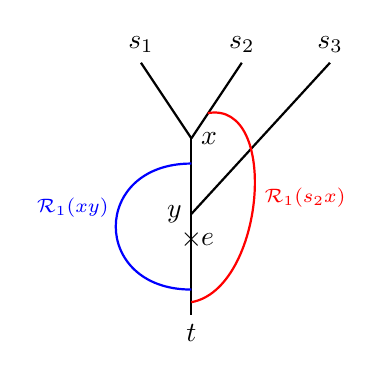
\begin{tikzpicture}[scale=1.6]
\begin{scope}
\coordinate (s2) at (0.4,2);
\coordinate (s1) at (-0.4,2);
\coordinate (s3) at (1.1,2);
\coordinate (x) at (0,1.4);
\coordinate (y) at (0,0.8);
\coordinate (t) at (0,0);
\coordinate (ts) at (0.15,0.4);
\coordinate (b1) at (0,.2);


\coordinate (a1) at (0,1.2);
\coordinate (a2) at (0.13,1.6);
\coordinate (v) at (0,.6);

\coordinate (c) at (-0.7,0.66);
\coordinate (b2) at (0,0.1);

\draw[thick](s1)--(x);
\draw[thick](s3)--(y);
\draw[thick](s2)--(x);
\draw[thick](x)--(t);
\node[above] at (s2){$s_2$};
\node[above] at (s1){$s_1$};
\node[above] at (s3){$s_3$};
\node[below] at (t){$t$};


\node[left] at (y){$y$};
\node[right] at (x){$x$};


\draw[blue,thick] (a1) to[out=180,in=180,distance=.8cm]
node[pos=0.4,left]
{\scriptsize  $\TON(xy)$}  (b1);



\draw[red,thick] (a2) to[out=10,in=10]
node[pos=0.5,right]
{\scriptsize  $\TON(s_2x)$}  (b2);

\node at (v){$\times$};
\node[right] at (v){$e$};

\end{scope}

\end{tikzpicture}
\caption{The shortest path from $s_2$ to $t$ avoiding $e$ can be $\TON(xy)$ or $\TON(s_2x)$.}
\label{fig:heavylight}

\end{figure}

\fi
\section{Building the Data Structure}
\iflong
\else
\vspace{-4mm}
\fi
\label{sec:data}

Let us first recognize a potential problem in using $\TON(\cdot)$.
%Consider a segment $xy$. We know that $\TON(xy)$ is a replacement path from $x$ to $t$ avoiding $yt_x$. We store only one path from $\TON$ for the segment $xy$   as
%we don't have enough space to store all the paths. However, this strategy leads to the following
%problem.
Let $s_1t$ and $s_2t$ path  meet at vertex $x$ (See Figure \ref{fig:heavylight}).
Another path $s_3t$
 meets $s_2t$ path at $y$ where $y$ is closer to $t$.
$\TON(s_2x)$ is the shortest path from $s_1$ to $t$ avoiding $e$ and $\TON(xy)$ is the shortest path from
$x$ to $t$ avoiding $e \in yt $. This immediately leads to the following problem. Assume that
the query is $\textsc{Q}(s_2,t,e)$ and the preferred path avoiding $e$ is in $\TON$.
Then there are two  candidate paths that avoid
$e$: one that goes from $s_2$ to the intersection vertex $x$ and then take
path  $\TON(xy)$ and the other $\TON(s_2x)$.
Thus, we need to check these two paths and return the minimum of the two. One can
make a bigger example in which there are $\sigma$ segments between $s_2$ and $t$
and thus we have to check $O(\sigma)$ path before we can answer the query. The problem appears
because we don't know from which segment the shortest path avoiding $e$ started its detour.
If this information is not there, then it seems that we have to look at all the segments between
$s_2$ ans $t$.
\iflong
\begin{figure}[hpt!]
\centering

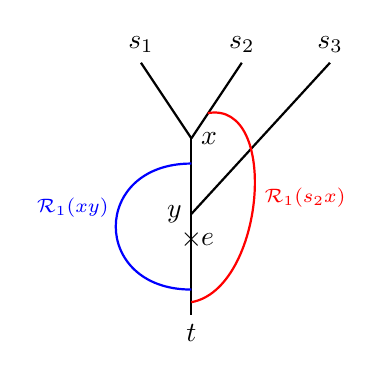
\begin{tikzpicture}[scale=1.6]
\begin{scope}
\coordinate (s2) at (0.4,2);
\coordinate (s1) at (-0.4,2);
\coordinate (s3) at (1.1,2);
\coordinate (x) at (0,1.4);
\coordinate (y) at (0,0.8);
\coordinate (t) at (0,0);
\coordinate (ts) at (0.15,0.4);
\coordinate (b1) at (0,.2);


\coordinate (a1) at (0,1.2);
\coordinate (a2) at (0.13,1.6);
\coordinate (v) at (0,.6);

\coordinate (c) at (-0.7,0.66);
\coordinate (b2) at (0,0.1);

\draw[thick](s1)--(x);
\draw[thick](s3)--(y);
\draw[thick](s2)--(x);
\draw[thick](x)--(t);
\node[above] at (s2){$s_2$};
\node[above] at (s1){$s_1$};
\node[above] at (s3){$s_3$};
\node[below] at (t){$t$};


\node[left] at (y){$y$};
\node[right] at (x){$x$};


\draw[blue,thick] (a1) to[out=180,in=180,distance=.8cm]
node[pos=0.4,left]
{\scriptsize  $\TON(xy)$}  (b1);



\draw[red,thick] (a2) to[out=10,in=10]
node[pos=0.5,right]
{\scriptsize  $\TON(s_2x)$}  (b2);

\node at (v){$\times$};
\node[right] at (v){$e$};

\end{scope}

\end{tikzpicture}
\caption{The shortest path from $s_2$ to $t$ avoiding $e$ can be $\TON(xy)$ or $\TON(s_2x)$.}
\label{fig:heavylight}

\end{figure}

\fi
To end this dilemma, we use heavy light decomposition of \SBFS($t$) \cite{SleatorT83}.
For any segment $xy \in$ \SBFS($t$) (by our convention $y$ is closer to $t$), $x$ is a {\em heavy}
child of $y$ if the number of nodes in the subtree under $x$ is $\ge$ 1/2(number of
nodes in the subtree under $y$) else it is called a {\em light child} (or light {\em segment} in our case).
%$x$ is also called the {\em heavy child} of $y$.
It follows
that each intersection vertex has exactly one heavy child and
each vertex is adjacent to atmost two heavy edges. A {\em heavy chain} is a concatenation of
heavy edges. A {\em heavy subpath} is a subpath of a heavy chain.
The following lemma notes a well known property of heavy-light decomposition.

\begin{lemma}
\label{lem:decomposition}
The path from a source $s$ to $t$ in \SBFS($t$) can be decomposed into $O(\log n)$ heavy subpaths
and light segments .
\end{lemma}

Given any source $s \in S$, by Lemma \ref{lem:decomposition},
the path from $t$ to $s$
may contain many heavy subpaths.
Let $C(pq)$ be a heavy
chain that starts at $p$
and ends at $q$ (where $q$ is closer to $t$ than $p$). A $ts$ path may follow
a heavy chain $C(pq)$ but may exit
this chain from a vertex midway, say at $r$. Let $(C(pq), r)$
be a tuple associated with $s$
such that the shortest path from $t$ to $s$ enters this
heavy chain via $q$ and
leaves this chain at $r$. We keep a list $\HE(s,t)$
which contains
all the tuples $(C(pq), r)$ sorted according to
the distance of heavy chain
from $t$ (that is distance $qt$). By Lemma \ref{lem:decomposition},
the size
of $\HE(s,t) = O(\log n)$. Similarly, we have one more
list to store the light segments.
$\LI(s,t)$ contains all the light segments on the $st$ path
again ordered according to their
distance from $t$ in \SBFS($t$). Again by Lemma  \ref{lem:decomposition},
the size
of $\LI(s,t) = O(\log n)$. Note that the size of these additional
two data-structures
is $\sum_{s \in S} O(\log n) = \tilde O(\sigma) = \tilde O(\sqrt{n\sigma})$.


Our main problem was that we have to find the minimum $\TON(\cdot)$ of $O(\sigma)$ segments if 
there is a path of length $\sigma$ between $s$ and $t$. The trick we use here is that
finding minimum on any heavy subpath takes $\tilde O(1)$ time. Since
there are $O(\log n)$ heavy subpaths, the total time taken to find the minimum
on heavy subpaths in $\tilde O(1)$. Also, since the number of light segments is also $O(\log n)$
finding the minimum among these also takes $\tilde O(1)$ time.

We now describe our intuition in detail.  Let $xy$ be a segment in a heavy chain
$C(pq)$. We want to represent $\TON(xy)$ in a
balanced binary search tree $\BST(C)$. To this end, we will add a node with
the tuple $(x.depth,| px \conc \TON(xy) |, |px|)$  in $\BST(C)$.
The first element in this tuple is the depth of $x$
in $\BFS(t)$ --  it also acts as the key in this binary search tree. The second element
is the path $ \TON(xy)$  concatenated with $px$. This concatenation is done so that all  paths
in $\BST(C)$ start from $p$ and comparing two paths in $\BST(C)$ is
possible. The third element will be used to get the path length $\TON(xy)$ (by subtracting it from
the second element) when
need arises. Now we can augment
this tree so that the following range minimum query can be answered in $\tilde O(1)$ time:
$\RMQ(C(pq),[a,b])$ : Find minimum of $\{|px \conc \TON(xy)|\ |\ xy \ \text{is a segment in heavy chain $C(pq)$ and }\ x.depth \ge a.depth \ \text{and}\  x.depth \le b.depth \}$.
The size of $\cup_{C \in \HE(s,t)}\BST(C)$ is $O(\sigma) = O(\sqrt{n\sigma})$ as there are
at most $O(\sigma)$ segments in \SBFS($t$).
\iflong
\begin{algorithm}
\SetKwRepeat{Do}{do}{while}%
  \caption{Finding the shortest replacement path  (in $\TON$) from $s$ to $t$ avoiding $e(u,v)$ }
  \label{fig:findR1R2}
Let $x$ be  the first intersection point on $us$ path\;
$min \leftarrow \infty$ \;

\Do{$x$ is not equal to $s$ }
{
    \If{ $x$ lies in a heavy chain}
    {
        Using $\HE(s,t)$, find $(C(pq),r)$, that is $r$ is the vertex from which $us$
        path leaves the chain $C$\;
        $min\leftarrow \min\{ min, \RMQ(C, [x,r]) - |pr| + |sr| \}$\;
        $x \leftarrow r$\;
    }
    \ElseIf{$x$ is an endpoint of a light segment}
    {
        Let $x'x$ be the  light segment ending at $x$ in \SBFS($t$) \tcp*{Can be found out via $\LI(s,t)$ in $\tilde O(1)$ time.}

        $min \leftarrow \min\{ min, |\TON(x'x)| + |sx'| \}$\;
        $x \leftarrow x'$\;
    }
}
\end{algorithm}
\fi


Given any edge $e(u,v)$ on $st$ path, we can now find the shortest path in $\TON$ from
$s$ to $t$ avoiding $e$
\iflong
(see Algorithm \ref{fig:findR1R2}).
\else
(Please refer to Algorithm \iflong\ref{fig:findR1R2}\else 1\fi~ in the full version of the paper).
\fi We first find the first intersection vertex on the
$us$ path from $u$. Let this vertex be $x$. We will see that finding
$x$ is also not a trivial problem --  we will say more about this problem later.
Now, we will go over all  possible replacement paths from $u$ to $s$.
Thus, we  search if there exists any heavy chain in
$\HE(s,t)$ that contains $x$. To this end, we first check if $x$ lies in some light segment (this can be checked in $\tilde O(1)$ time). If not, then $x$ lies in some heavy chain. We now search each heavy chain in $\HE(s,t)$ to find a node $x'$ with the smallest depth such that  $x'.depth > x.depth$.
Let this node be $x'$. Thus we have found the segment $x'x$ where $x$ is closer to $t$
than $x'$.
%where $x.depth$ is the depth of $v$ in $\BFS(t)$.
We can easily calculate $x.depth$ as
$|st| - |sx|$ or $B_0(s,t) - B_0(s,x)$. Since there are $\tilde O(1)$ heavy
chain in $\HE(s,t)$, the time taken to find if $x'x$ exists in some heavy chain is $\tilde O(1)$.
%Similarly, the reader can infer that the time taken to %find the light segment
%in which $x$ is an endpoint is $\tilde O(1)$.
%Once we have found such a
%heavy path or light segment, then we check if the replacement %lies on it.

Assume that we found out that
$x'x \in C(pq)$,  and $ts$ path leaves the chain $C$ at $r$, then we want to
find the shortest replacement path from $r$ to $t$ avoiding $e$. This can be found out via the range minimum query $\RMQ(C(p,q),[x,r])$.
However, note that each replacement path in $C$ starts from $p$. So, we need to
remove $|pr|$ from the replacement path length returned by $\RMQ$ query.
The length $pr$ can be found out in the node $r \in \BST(C)$. Finally, we add $|sr|$ to get the path from $s$ to $t$.

Similarly, we can process a light segment in $O(1)$ time (please refer to Algorithm \iflong\ref{fig:findR1R2}\else
1 in the full version\fi~).
Thus, the time taken by  Algorithm  \iflong\ref{fig:findR1R2}\else
1\fi~ is
$\tilde O(1)$ as the while loop runs at most $O(\log n)$ times  and each step in
the while loop runs in $\tilde O(1)$ time.



%The above algorithm moves from vertex $u$ to $s$, that is $us$ path.
%If it encounters a light edge $vv'$ in this path then it, then we check if the
%$st$ path whose detour starts on $vv'$ is the minimum, that is path $sv' \conc \TON(v')$.
%Else, if we encounter a heavy chain, then we

\begin{comment}
We are now ready to describe our data-structure to process queries. We first need
to check the vertex to be avoided is an intersection point in \SBFS$(t)$. To this end,
we check if the vertex exists in $\BST_1(t)$. If yes, then we return the length of the
preferred path associated with the vertex. The size of
$\BST_1(t)$ is $O(\sigma) = O(\sqrt{n \sigma})$ as there are $O(\sigma)$ intersection
point in \SBFS$(t)$.


Let $xy$ be a segment in \SBFS$(t)$.  We will associate two data structures with
$x$, (1) $D_0(x,t)$ contains   the preferred replacement path from $x$ to $t$
such that its detour starts in segment $xy$, but the avoided vertex lies in $yt$,
that is, that path in $\TON$ (2) $\BST_2(x,t)$ contains all the  preferred path
from $x$ to $t$ such that their detour start in segment $xy$ and the avoided
vertex also lies in $xy$, that is, paths in $\TTW$. As in the single source case,
we first show that each path in $\BST_2(x,t)$ avoid a contiguous subpath of $xy$.

By Corollary \ref{cor:arrange}, we can arrange paths in $\BST_2(x,t)$ in decreasing order of their length. By
Lemma \ref{lem:avoids}, for any two path $P,P' \in \BST_2(x,t)$, if $|P| > |P'|$, then $\DET(P')$
starts below the vertex avoided by $P$. This lemma implies
that $\DET(P')$ starts below all the vertices avoided by
$P$. Thus $P$ avoids some contiguous path in $xy$ path.
We can $\BST_2(x,t)$ as a balanced binary search tree. For each subpath $zz'$ of $xy$,
we store the length of the replacement path from $x$ whose detour starts before $z$ and it
meets $xt$ path again in $t_xt$.  Additionally, we also store the distance of $z$ and $z'$
from $x$. These distances will act as the key of a node in $\BST_2(x,t)$.
\end{comment}
\iflong
\else
\vspace{-2mm}
\fi
\subsection{Answering queries in $\tilde O(1)$ time}
\iflong
\else
\vspace{-2mm}
\fi
Given a query ${\sc Q}(s,t,e(u,v))$, we process it as follows
(assuming that $e$ lies on $st_s$ path (that is the {\em far case)} and $v$ is closer to $t$ than $u$)\iflong\\\else\vspace{1mm}\fi


\begin{comment}
{\em (1) Check if $e$ lies on $st_s$ path.}

  Since all the shortest path have unique length, we find if $|su|_{p} + |ut_s| _{p}+ |t_st|_{p} = |st|_p$. To this end, we use the data structure already defined in Section \ref{}. We first find $t_s \leftarrow
  B_2(s,t)$.
  Then we check if $B_0^{p}(s,u) +\ B_0^{p}(u,t_s) +\ B_0^{p}(t_s,t)
  = B_0^{p}(s,t)$.

  \item Check if $u$ is an intersection vertex in \SBFS$(t)$.

  For each $t$ we build a balanced binary search tree that stores all the intersection vertex in $\BFS(t)$. Since the number of intersection vertex in $\BFS(t)$ is $O(\sigma)$, the size of this binary search tree is $O(\sigma) = O(\sqrt{n \sigma})$. We then check now check  $u$ is an intersection vertex in  $\tilde O(1)$ time.

\end{comment}

\begin{enumerate}[leftmargin=*,noitemsep,nolistsep]
\item Find the first intersection vertex  on $us$ path.

\iflong
  \noindent As we have mentioned before, this is not a trivial problem.
  Let the first intersection vertex from $u$ to $s$ in $\BST(t)$ be
  denoted by  $\INT_{s}(u,t)$.   We will first show that $\INT_{s}(u,t)$ is independent of $s$.
  \begin{lemma}
  \label{lem:intlemma}
  $\INT_s(u,t) = \INT_{s'}(u,t)$ for $s,s' \in S$ for all $u \in \BFS(t)$.
  \end{lemma}

  \iflong
  \begin{proof}
    We will prove this by induction on the nodes of $\BFS(t)$ from leaf to root $t$.
    The base case is a leaf in $\BFS(t)$, that is a source vertex, which by definition,
    itself is an intersection vertex. For any node $u$, if $u$ is an intersection vertex,
    $\INT_s(u,t) = \INT_{s'}(u,t) = u$. Else, $u$ is a node of degree 2 in $\BFS(t)$.
    Assume that $u'$ is the child of $u$ in $\BFS(t)$. So, $\INT_s(u,t) = \INT_s(u',t)$ and $\INT_{s'}(u,t) = \INT_{s'}(u',t)$. But by induction hypothesis,  $\INT_s(u',t)=\INT_{s'}(u',t)$.

    \end{proof}
  \fi

  \noindent We will drop the subscript $s$ from the definition of $\INT(\cdot,\cdot)$ as we now know that it is independent of $s$. We use the
  above lemma to construct  two data structures that will help us in finding $\INT(u,t)$.

  \begin{itemize}
  \item $I_1(t)$: For any $u \in V$, if $\INT(u,t)$ is within a distance of $c\sqrt{n/\sigma} \log n$
  (for some constant $c$) from $u$, then we store the tuple
  $(u,\INT(u,t)$) in the balanced binary search tree $I_1(t)$. For any  intersection
  vertex $x \in $ \SBFS$(t)$, we  store at most $\tilde O(\sqrt{n/\sigma})$ tuples in $I_1(t)$.
  For a fixed $t$, the total
  space taken by $I_1(t)$ is $\tilde O(\sigma .\sqrt{(n/\sigma)}
  )= \tilde O(\sqrt{n \sigma})$ (as there are $O(\sigma)$ intersection vertices in \SBFS($t)$.
  %Given a vertex $u$, we then try to find if $u$
  %exists in this data-structure. This takes $\tilde O(1)$
  %time.

  \item $I_2(t)$: If $u$ is not present in $I_1(t)$, then $\INT(u,t)$ is at a distance
  $\ge c\sqrt{n /\sigma}\log n$ from $u$. We now
  use a different strategy to find $\INT(u,t)$. We first find $u_s \leftarrow B_1(s,u)$,
  that is the vertex in $\TT$
  closest to  $u$ in $su$ path. With a
high probability,
$u_s$ is closer to $u$ than $\INT(u,t)$ and all the vertices from $u$ to $u_s$ have degree  exactly 2 in $\BFS(t)$.
  Thus, $\INT(u_s,t) = \INT(u,t)$ -- we will now use this property (a similar property was also used in the proof of Lemma \ref{lem:intlemma}).

  \begin{comment}
        \begin{figure}[hpt!]
        \begin{algorithm}[H]
        \If{$u \in I_1(t)$}
        {
            return $I_1(u,t)$;
        }
        \Else
        {
            $u_s \leftarrow B_1(s,u)$\;
            return $I_2(u_s,t)$;
        }
        \end{algorithm}
        \caption{\textsc{Find-Int}$(s,u,t)$: An algorithm to find $\INT_s(u,t)$}
        \end{figure}
  \end{comment}
  \noindent
  For each $x \in \TT$
  such that $x$ is not an intersection vertex in $\BFS(t)$, we store the tuple
  $(x,\INT(x,t))$ in another balanced binary search tree $I_2(t)$. For a fixed vertex $t$, the
  size of this data-structure is $\tilde O(\sqrt{n\sigma})$ space
  as there is only one intersection vertex for each vertex
  in $\TT$ and $|\TT| = \tilde O(\sqrt{n \sigma})$

\end{itemize}
  \noindent If $\INT(u,t)$ is indeed at a distance $\le
c \sqrt{n / \sigma} \log n$,
  then we can use $I_1(t)$  to find it in $\tilde O(1)$
time, else we use $I_2(t)$ to find
  $\INT(u_s,t)$ in $\tilde O(1)$ time.\\

  \begin{comment}
  \noindent {\em Assuming $x = \INT_s(u,t)$,  find $\INT_s(x,t)$}

  Our aim is to find the segment which ends at $x$ in \SBFS($t)$. To this end,
  we find $\INT(x,t)$. To this end, we use another balanced binary search tree.
  For each intersection vertex $v \in $ \SBFS($t$), we store the tuple
  $(s,\INT_s(v,t))$ in $I_3(v,t)$. Unlike non intersection vertex, for an
  intersection vertex $v$, $\INT_s(v,t)$ may be dependent on $s$.

  \end{comment}
\else
\noindent In the full version of the paper, we show that we can find the first intersection vertex  on $us$ path
in $\tilde O(1)$ time using $O(\sqrt{n\sigma} )$ space.
\fi
\item Find  the replacement path avoiding $u$  if it lies in $\TON$.
\label{fcase1}

\noindent To this end, we use our Algorithm \iflong\ref{fig:findR1R2}\else
1\fi.
The first non-trivial part of this algorithm, that is, finding the first
intersection vertex on the $us$ path has already been tackled in the point above.
So we can find such a replacement path (if it exists) in
$\tilde O(1)$ time  and $\tilde O(\sqrt{n \sigma})$ space.\iflong\\\else\vspace{1mm}\fi


\item Find the replacement path avoiding $e(u,v)$ if it lies in $\TTW$.
\label{fcase2}

\noindent  This part is similar to our data-structure in single source case.
Let $x \leftarrow \INT(u,t)$.  Using $\HE(s,t)$ and $\LI(s,t)$, in $\tilde O(1)$ time,
we can find the segment $xy \in $ \SBFS($t$) such that $y$ is closer to $t$ than $x$.
In this case, we want to check if there exists any
replacement path that starts in  the  same segment in which
$e$ resides. This  replacement path first takes $sx$ path and then takes
 the  detour strictly inside  the  segment $xy$. All such paths are stored in $\TTW(xy)$
with the contiguous range of edges that they avoid on $xy$.
We now just need to check if $u$ and $v$ lie in the range of some replacement path.
To this end, we find $u.depth \leftarrow |st| -|su| = B_0(s,t) - B_0(s,u)$
and $v.depth \leftarrow |st| -|sv| = B_0(s,t) - B_0(s,v)$.
Now we check if $u.depth$ and $v.depth$ lie in contiguous range of
some replacement path  in $\TTW(xy)$. If yes, then we return the length of that
path concatenated with $sx$.  Note that we have already stored $|sx|$ in $B_0(s,x)$.
The time taken in this case is dominated by searching $u$ and $v$ in $\TTW(xy)$,
that is $\tilde O(1)$.\iflong\\\else\vspace{1mm}\fi
\end{enumerate}

\noindent Thus, the total query time of our algorithm is $\tilde O(1)$, and we can return the
minimum of replacement paths found in Step \ref{fcase1} and \ref{fcase2} as our final answer.
The reader can check that the space taken by our algorithm for a
vertex $t$ is $\tilde O(\sqrt{n\sigma})$. Thus the total space taken by our algorithm is
$\tilde O( \sigma^{1/2} n^{3/2}) $. Thus we have proved the main result, that is Theorem \ref{thm:maintheorem} of our paper.

%\begin{theorem}
%There exists a data-structure of size $\tilde O(\sigma^{1/2}n^{3/2})$
%for multiple source single fault tolerant exact distance oracle
%that can answer each query in $\tilde O(1)$ time.
%\end{theorem}


\bibliographystyle{plain}
\bibliography{sample}

\end{document}
